\documentclass[12pt]{article}
\textwidth=6.3in
\voffset= -2cm
\hoffset= -1.3cm
\textheight=23.5cm


\usepackage{amssymb, amsmath, amscd}
\usepackage{graphicx}
\usepackage[latin1]{inputenc}
%\usepackage{natbib}
\usepackage{epsfig}
\usepackage{color}


% THEOREMS -------------------------------------------------------
\newtheorem{definition}{Definition}
\newtheorem{postulate}{Postulate}
\newtheorem{theorem}{Theorem}
\newtheorem{proposition}{Proposition}
\newtheorem{lemma}{Lemma}
\newtheorem{corollary}{Corollary}
%\newtheorem{proof}{Proof}
\newtheorem{notation}{Notation}
\numberwithin{equation}{section}

\usepackage{pdflscape}
\usepackage{afterpage}
\usepackage{capt-of}
% ----------------------------------------------------------------
\begin{document}
% MACROS article ISSAC 2007
% ---------------------

%\usepackage{calc}
%\usepackage{amsthm, amsmath}
%\usepackage{amssymb}

%%%%%% lettres caligraphiques
\newcommand{\calA}{{\cal A}}
\newcommand{\calB}{{\cal B}}
\newcommand{\calF}{{\cal F}}
\newcommand{\calG}{{\cal G}}
\newcommand{\calR}{{\cal R}}
\newcommand{\calZ}{{\cal Z}}
\def\D{\mathcal{D}}
\def\L{\mathcal{L}}
\def\S{\mathcal{S}}
\def\I{\mathcal{I}}
\def\V{\mathcal{V}}
\def\E{\mathcal{E}}
\def\M{\mathcal{M}}


\def\A{\mathscr{A}}
\def\F{\mathscr{F}}
\def\G{\mathscr{G}}


%%%%%% Ensembles de nombres
\newcommand{\N}{{\mathbb N}}
\newcommand{\Z}{{\mathbb Z}}
\newcommand{\Q}{{\mathbb Q}}
\newcommand{\R}{{\mathbb R}}
\newcommand{\CC}{{\mathbb C}}

\newcommand{\K}{{\mathbb K}}
\newcommand{\kk}{{\mathrm k}}

%%%%%%  mathrm
\def\J{\mathrm{J}}
\def\catC{{\bf \mathrm{C}}}
\def\x{\mathrm{x}}
\def\a{\mathrm{a}}
\def\d{\mathrm{d}}
\def\Bi{\mathrm{Bi}}
\def\op{\mathrm{op}}
\def\res{\mathrm{res}}
\def\span{\mathrm{span}}

\newcommand{\C}{{\bf C}}
\newcommand{\Objects}{{\bf Objects}}
\newcommand{\Arrows}{{\bf Arrows}}
\newcommand{\Sets}{{\bf Sets}}

%%%%% hypergoemetric functions
\def\2F1{\mbox{ $_2${F}$_1$}}
\def\1F1{\mbox{ $_1${F}$_1$}}
\def\1F2{\mbox{ $_1${F}$_2$}}
\def\0F1{\mbox{ $_0${F}$_1$}}

%%%%% Groupes
\def\GL{\mathrm{GL}}
\def\det{\mathrm{det}}
\def\SL{\mathrm{SL}}
\def\PSL{\mathrm{PSL}}
\def\PGL{\mathrm{PGL}}
\def\O{\mathrm{O}}

%%% Algebres de Lie
\def\gl{\mathfrak{gl}}
\def\g{\mathfrak{g}}
\def\h{\mathfrak{h}}
\def\frakM{\mathfrak{M}}

\newcommand{\Frac}[2]{\displaystyle \frac{#1}{#2}}
\newcommand{\Sum}[2]{\displaystyle{\sum_{#1}^{#2}}}
\newcommand{\Prod}[2]{\displaystyle{\prod_{#1}^{#2}}}
\newcommand{\Int}[2]{\displaystyle{\int_{#1}^{#2}}}
\newcommand{\Lim}[1]{\displaystyle{\lim_{#1}\ }}

% systemes d'equations
\newenvironment{menumerate}{%
    \renewcommand{\theenumi}{\roman{enumi}}%
    \renewcommand{\labelenumi}{\rm(\theenumi)}%
    \begin{enumerate}} {\end{enumerate}}

\newenvironment{system}[1][]%
	{\begin{eqnarray} #1 \left\{ \begin{array}{lll}}%
	{\end{array} \right. \end{eqnarray}}

\newenvironment{meqnarray}%
	{\begin{eqnarray}  \begin{array}{rcl}}%
	{\end{array}  \end{eqnarray}}

\newenvironment{marray}%
	{\\ \begin{tabular}{ll}}
	{\end{tabular}\\}

\newenvironment{program}[1]%
	{\begin{center} \hrulefill \quad {\sf #1} \quad \hrulefill \\[8pt]
		\begin{minipage}{0.90\linewidth}}
	{\end{minipage} \end{center} \hrule \vspace{2pt} \hrule}

\newcommand{\entrylabel}[1]{\mbox{\textsf{#1:}}\hfil}
\newenvironment{entry}
   {\begin{list}{}%
   	{\renewcommand{\makelabel}{\entrylabel}%
   	  \setlength{\labelwidth}{40pt}%
   	  \setlength{\leftmargin}{\labelwidth + \labelsep}%
   	}%
   }%
   {\end{list}}

\newenvironment{remark}{\par \noindent {\bf Remark. }}
			{\hfill $\blacksquare$ \par}
\newenvironment{example}{\par \noindent {\bf Example. }}
			{\hfill $\blacksquare$ \par}

\newenvironment{Pmatrix}
        {$ \left( \!\! \begin{array}{rr} }
        {\end{array} \!\! \right) $}



%%%%% Abbreviations
\newcommand{\fleche}[1]{\stackrel{#1}\longrightarrow}
\def\ssi{si et seulement si\ }
\newcommand{\tab}{\hspace*{\fill}}
\newcommand{\bs}{{\backslash}}
\newcommand{\eps}{{\varepsilon}}
\newcommand{\into}{{\;\rightarrow\;}}
\newcommand{\PD}[2]{\frac{\partial #1}{\partial #2}}
\def\Hat{\widehat}
\def\Bar{\overline}
\def\vect{\vec}
\def\fbar{{\bar f}}
\def\xbar{{\bar \x}}
\newcommand{\afaire}[1]{$$\vdots$$ \begin{center} {\sc #1} \end{center} $$\vdots$$ }
\newcommand{\pref}[1]{(\ref{#1})}

\def\Maple{{\sc Maple}}
\def\RG{{\sc Rosenfeld-Gr\"obner}}


%%%% Algos
%\newcommand{\algf}{\sffamily}
%\newcommand{\FUNCTION}{{\algf fonction}}
%\newcommand{\BEGIN}{{\algf debut}}
%\newcommand{\END}{{\algf fin}}

%\newcommand{\IF}{{\algf si}\ \ \ \=\+}
%\newcommand{\THEN}{{\algf alors}\ }
%\newcommand{\ELSE}{\=\-\kill{\algf sino}\=\+{\algf n}}
%\newcommand{\ELIF}{{\algf sinon}\=\+{\algf si}\ }
%\newcommand{\FI}{\=\-\kill{\algf fin si}\ }
%\newcommand{\FOR}{{\algf pour}\ \=\+}
%\newcommand{\ENDFOR}{\=\-\kill{\algf fin pour}\ }
%\newcommand{\FROM}{{\algf de}\ }
%\newcommand{\TO}{{\algf \a`a}\ }
%\newcommand{\WHILE}{{\algf tq}\ \ \ \=\+}
%\newcommand{\ENDWHILE}{\=\-\kill{\algf fin tq}}
%\newcommand{\DO}{{\algf faire}\ }
%\newcommand{\OD}{{\algf od}}
%\newcommand{\RETURN}{{\algf retourner}}
%\newcommand{\INDENTER}{{\algf si} \=\+\kill}


\newcommand{\algf}{\sffamily}
\newcommand{\BEGIN}{{\algf begin}}
\newcommand{\END}{{\algf end}}
\newcommand{\IF}{{\algf if}}
\newcommand{\THEN}{{\algf then}}
\newcommand{\ELSE}{{\algf else}}
\newcommand{\ELIF}{{\algf elif}}
\newcommand{\FI}{{\algf fi}}
\newcommand{\WHILE}{{\algf while}}
\newcommand{\FOR}{{\algf for}}
\newcommand{\DO}{{\algf do}}
\newcommand{\OD}{{\algf od}}
\newcommand{\RETURN}{{\algf return}}
\newcommand{\PROCEDURE}{{\algf procedure}}
\newcommand{\FUNCTION}{{\algf function}}
\newcommand{\INDENTER}{{\algf si} \=\+\kill}

%% Op�rateurs
\newcommand{\target}{\mathop{\mathrm{t}}}
\newcommand{\source}{\mathop{\mathrm{s}}}
\newcommand{\trdeg}{\mathop{\mathrm{tr~deg}}}
\newcommand{\jet}[2]{\jmath_{#1}^{#2}}
\newcommand{\rank}{\operatorname{rank}}
\newcommand{\sign}{\operatorname{sign}}
\newcommand{\ord}{\operatorname{ord}}
\newcommand{\aut}{\operatorname{aut}}
\newcommand{\Hom}{\operatorname{Hom}}
\newcommand{\myhom}{\operatorname{hom}}
\newcommand{\codim}{\operatorname{codim}}
\newcommand{\coker}{\operatorname{coker}}
\newcommand{\rp}{\operatorname{rp}}
\newcommand{\leader}{\operatorname{ld}}
\newcommand{\card}{\operatorname{card}}
\newcommand{\Fr}{\operatorname{Frac}}
\newcommand{\RF}{\operatorname{\mathsf{reduced\_form}}}
\newcommand{\rang}{\operatorname{rang}}

\def \Id{\mathrm{Id}}
%\def \span{\mathrm{span}}

\def \diff{\mathrm{Diff}^{\mathrm{loc}} }
\def \diffg{\mathrm{Diff} }
\def \Esc{\mathrm{Esc}}

\newcommand{\initial}{\mathop{\mathsf{init}}}
\newcommand{\separant}{\mathop{\mathsf{sep}}}
%\newcommand{\rem}{\mathop{\mathsf{rem}}}
\newcommand{\quo}{\mathop{\mathsf{quo}}}
\newcommand{\pquo}{\mathop{\mathsf{pquo}}}
\newcommand{\lcoeff}{\mathop{\mathsf{lcoeff}}}
\newcommand{\mvar}{\mathop{\mathsf{mvar}}}

\newcommand{\prem}{\mathop{\mathsf{prem}}}
\newcommand{\remp}{\mathrel{\mathsf{partial\_rem}}}
\newcommand{\remf}{\mathrel{\mathsf{full\_rem}}}
\renewcommand{\gcd}{\mathop{\mathrm{gcd}}}
%\renewcommand{\deg}{\mathop{\mathrm{deg}}}
\newcommand{\pairs}{\mathop{\mathrm{pairs}}}
\newcommand{\dd}{\mathrm{d}}
\newcommand{\ideal}[1]{(#1)}
\newcommand{\cont}{\mathop{\mathrm{cont}}}
\newcommand{\pp}{\mathop{\mathrm{pp}}}
\newcommand{\pgcd}{\mathop{\mathrm{pgcd}}}
\newcommand{\ppmc}{\mathop{\mathrm{ppcm}}}
\newcommand{\init}{\mathop{\mathrm{initial}}}


\bibliographystyle{abbrv}

%\title{Quantum topological de novo discovery of mutated driver pathways in cancer}
\title{Topological and quantum tools for \\ {\it de novo} mutated driver pathways discovery in cancer}
%\title{{\sc Topological approach to cancer genomics pathways}
\author{Raouf D  - joint work Hedayat Alghassi\\
%\small{{\sc 1QB Information Technologies (1QBit)}}
}
  \date{\today}
\maketitle

%\tableofcontents

%\begin{abstract}
%~~\\
%	 It has been recognized that a key step towards defeating cancer is a deep understanding of the genomic  changes that occur before and during the tumorgenesis.    	%The translation of any deep understanding into therapies
%	%is not the purpose of this work.
%	 Our work attempts to contribute to this understanding through the proposal of a novel topological framework and   
%	  to introduce the use of quantum annealing to help with large scale computations one faces 
%	in genomic data analysis. 
%	 We hope that, within this framework and armed with the computational capabilities of quantum computers, a new type of questions about the data can be asked i.e., a different kind of hypotheses can be formulated. We have
%	   used in our analysis real (TCGA) mutation data of two types of tumour:  Acute myeloid leukemia and Glioblastoma multiform.   As a first application, we  explain how the noisy data problem in the data-driven pathways discovery is dealt with within this framework using  persistent homology. 
%	   We present a complete persistent homology-based algorithm built on the top of our quantum procedure.  For both datasets, using our  homology based  quantum pipeline, we have recovered the same pathways previously found in addition to new additional pathways. 
%	   
%	   \medskip
%	
%	~~\\
%	
%	   \medskip   
%	   
%%	   {\it ``How can it be that mathematics, being after all a product of human thought which is independent of experience, is so admirably appropriate to the objects of reality?" [Albert Einstein]}
%%
%%	{\it ``We should stop acting as if our goal is to author extremely elegant theories, and instead embrace complexity and make use of the best ally we have: the unreasonable effectiveness of data." [Peter Norvig]}
%	
%\end{abstract}	  

%{\color{blue} Cite "Topology and data" and "Ayasdi work in breast cancer" }
%	 ~~\\
	 
	 	 ~~\\		 
{\bf Key words:} {\it  Cancer genomics, mutation data,  acute myeloid leukemia, glioblastoma multiform, quantum computers, persistent homology, topological data analysis. }
  
%  \section*{Contributions highlight}
%  \begin{itemize}
%  	\item[1] We propose a quantum procedure for the {\it de novo} discovery of mutated driver pathways in cancer. We have tested our procedure on D-Wave  quantum processor.
%	\item[2] We propose the use of the so-called persistent homology for fine tuning the output of our quantum procedure. This is particularly useful since mutation data is often noisy due to errors occurring during the sequencing or/and in  the different steps of preparing the data.
%	\item[3] The third contribution is the introduction of the mathematical concept of ``space of pathways". In fact, it plays an important role in 
%2 above but as a tool or a construction. We have tried to  go beyond that and explored it as concept in a way  
%{closer to the ``integrated circuit of the cell" picture  of \cite{hallmarksOfCancer}}.      We hope (as we usually do in topological data analysis) that the  global topological  properties of this space translate into new insights on how mutations work together in  affecting the relevant pathways  and causing cancer.  Exploring the usefulness of this approach (i.e., biological validation of the approach for which we have some finding - see Conclusion)  is under investigation and is the ultimate goal
%of this topological investigation.
%  \end{itemize}
%  
%  \section*{What I feel needs to be done}
%[This is not part of the paper - it is here to share with Gordon what I think is missing]  The paper proposes flexible frameworks and introduces powerful techniques. All of that is very much welcome (as Gordon noticed) but still, in my opinion,  it is a mathematical proposal with a {\it naive} biological connection/validation/raison d'�tre. I like to strengthen this connection; I would like to fine tune the mathematics we present (which I am happy with) as much as possible (by directing it to a more sophistical biological question(s)) so it makes sense for at least bioinformaticians. I would be happy if someone like Ben Raphael reads the paper and finds it really interesting and relevant to the field. 


%  \section*{Introduction}
~~\\
Cancer is driven by somatic mutations that target signalling and regulatory pathways that control cellular proliferation and cell death~\cite{bioOfCancer}. Understanding how this happens is of paramount importance 
in order to improve our ability to intervene and attack cancer.

~~\\
Since  the advent  of DNA sequencing technologies, our understanding has progressed enormously.  Current advances range from the introduction of a single anti-cancer agents, which simply bind with growth factor receptors stopping abnormal cell 
proliferations (For instance, in the context of  breast cancer, 
  Herceptin antibody stops cells abnormal proliferation signals by binding  with the excess of growth factor receptors on the cell surface  caused by point mutations in the gene Her2.   Gleevec  is a second example. It is used to treat  chronic myeloid leukemia which is a type of blood cell tumour due to an inappropriate gene fusion product
of a translocation in chromosomes 9 and 22. The resulting fusion gene BCR-ABL has an increased kinase activity resulting an increase in 
proliferation signals.  Similarly to Herceptin, Gleevec blocks the growth signals the abnormal fusion gene generates and thus prevents the cell proliferation) to more sophisticated approaches such as immunotherapy which activates  the immune system against cancer cells  and as well as the use of combinations of therapeutic agents to
attack multiple pathways fundamental in cancer development, preventing resistance from occurring.  %But, much more work remains to be done.


%For example, recent researches have led to the ability to activate the immune system against cancer cells.  Called immunotherapy, this approach has shown success with melanoma, leukemia, and lymphoma, and is ripe for further exploration in a wider range of cancers.  Another approach attacks multiple pathways fundamental in cancer development, using combinations of therapeutic agents to prevent resistance from occurring.  %But, much more work remains to be done.


%This led to  the introduction of very efficient molecularly target anti-cancer agents. 

~~\\
 Sadly, cancer morbidity is still  very high and
 our understanding is still incomplete particularly for the advanced stages of the tumorigenesis.  As mathematicians and scientists in computation, we are concerned about two reasons related to this limitation: 1) not all relevant pathways have been identified 2) and more fundamentally, we don't know how these mutations
 affecting different pathways work together to cause cancer.  
 
 ~~\\
 The work discussed in the present paper is part of our series of two papers which intent to join efforts in elucidating these two problems in particular. The other
 paper of this series is \cite{raoufQubo}.   Our contribution  is threefold: 
 \begin{itemize}
\item [1] It is a fact that the computational determination of pathways   is  expensive and beyond the capabilities 
		of classical computers. For this reason we have started our investigation by explaining  how quantum computers can be used.  
		We propose a new quantum procedure  \cite{raoufQubo} which we have tested on D-Wave 2X quantum processor.
		This is in addition to simplicial complexes  construction algorithms discussed in \cite{raoufHomology} (the connection
		between simplicial complexes and pathways is introduced below).
 
\item [2] It is also a fact that, due to errors occurring during the sequencing or/and in  the different steps of preparing the data, mutation data is often noisy.
Our second contribution is the introduction of  topological analysis for fine tuning  our quantum procedure \cite{raoufQubo} for a more robust outcome. 
The technique we have used is called persistent homology and is a powerful tool in topological data analysis~\cite{MR2476414}.  
 
\item [3] The third contribution is the introduction of the mathematical concept of ``space of pathways". In fact, it plays an important role in 
2 above but as a tool or a construction. We have tried to  go beyond that and explored it as concept in a way  
{closer to the ``integrated circuit of the cell" picture  of \cite{hallmarksOfCancer}}.      We hope (as we usually do in topological data analysis) that the  global topological  properties of this space translate into new insights on how mutations work together in  affecting the relevant pathways  and causing cancer.  Exploring the usefulness of this approach (i.e., biological validation of the approach for which we have some finding - see Conclusion)  is under investigation and is the ultimate goal
of this topological investigation.
%Such structural investigation might also help in the quest for  some sort of  {\color{blue} selectivity} aiding, for instance, 
%chemotherapeutic agents in targeting tumour cell efficiently without harming normal neighbouring cells. Our model is flexible and can be improved by constantly confronted  with new experimental results and can  tweaked to better capture these results.   {\color{blue} Weinberg picture of electric circuits -The Hallmarks of cancer}
	
% We argue that this transition not only (1)  opens  the door for us to utilize the sophisticated  algebraic machinery which comes along with this perspective (eg., persistent homology showcased in Section~2 where we tackle the noise in the data) but also (2) provides a new framework where a different type of data analysis hypotheses can be formulated (showcased in the conclusion by an open question).	
\end{itemize}
%It is correct to think about the first two items as collecting the pieces of the puzzle while the last item is helping solving the puzzle
%by probing the   space of pathways.
The first contribution has been detailed and compared to other available approaches in \cite{raoufQubo}.  
 The last two  are the subject of the present paper  which we now outline its main ideas. 
Our topological journey departs from the fact  that signalling or regulatory  pathways  are in fact independent sets (modulo 
some notion of tolerance introduced in the next Section to accommodate noise in the data as well as potential interactions between pathways constituents such as crosstalk and synthetic lethality)
and thus when grouped together they define  a {\it simplicial complex} (i.e., a collection of objects called {\it faces} closed under some boundary map  i.e., the boundary of a face is again a face. 
 A clique (resp. independence)  complex of a graph $G$ is a simplicial complex whose faces 
are cliques  (resp. independent sets)  of $G$ and boundary map is the inclusion of sets) . This vantage point connects us to the marvellous world of topology where simplicial complexes are  the prototypes of  spaces with shapes. Our journey is all about  exploring the usefulness of this notion of shape in cancer genomics.  In fact, all what is presented here (point 2 and 3 above) is articulated around  the sequence of assignments: 

 ~~\\ 
  \begin{tabular}{ccccccc}\label{functor3}
	{\bf mutationData} & 		$\rightarrow$      & {\bf graphs} & $\rightarrow$& {\bf SpaceOfPathways}  		& $\rightarrow$& {\bf ShapeMeasurements} \\\nonumber
	$X$ 			   &           $\mapsto$ 	 &   $G$            &$\mapsto$  &    $ \mathcal N(K)$                             &$\mapsto$ &      $H_*(\mathcal N(K))$\\
\end{tabular}
%
%
%\begin{eqnarray}\label{functor3}
%	{\bf mutationData} & 		\rightarrow& 		{\bf graphs} \rightarrow {\bf simplicialComplexes}  			j\\\nonumber
%	X 			   &\mapsto 		&              \quad G \quad   \quad \mapsto  \mathcal N(K)  \quad \qquad \mapsto \\
%\end{eqnarray} 

~\\
where: 
\begin{itemize}
\item $G$ is the mutation graph i.e., 
is the graph defined by the set of genes in $X$  where two genes are connected if they have harboured mutations for the same patients.
  $K$ is the simplicial complex  given by the set of all independent sets of $G$.  It is important to mention again that the construction of the simplificial complex $K$ is prohibitively hard task for classical computers. This is where our quantum algorithm
 is used. The underlying mathematics detailed in \cite{raoufHomology} is based on the so-called Mayer-Vietoris construction which itself is articulated around clique covering the graph $G$. We prove in \cite{raoufHomology}  that for a large class of graphs, a such covering provides most of the simplices of $K$.  Another quantum approach which can be used here as well is the quantum algorithm presented in \cite{seth} written in the gate model (our is written as
an adiabatic quantum computation). 
\item $  \mathcal N(K)$ is the space of pathways. The facets (maximal independent sets) of $K$ are the pathways and their nerve defines the {space of pathways} $  \mathcal N(K)$ (pictorially, 
the space of pathways is visualized through its 1-skeleton: the graph with pathways as vertices and two pathways
are connected if they intersect. Precise definition is in the text). 
\item $H_*(\mathcal N(K))$  is the homology of  the space of pathways i.e., the shape measurements of the space of pathways (definition in the text). 
\end{itemize}




	 
	 ~~\\
	 We have applied our approach to two different   TCGA
	 mutation data: Acute myeloid leukemia (AML) \cite{doi:10.1056/NEJMoa1301689} and Glioblastoma multiform (GBM) \cite{GBM2008}. For both the data,
	 we have computed the assignment tumour $\mapsto$ space of pathways using persistent homology.  Interestingly, our calculation also shows  that the space of pathways for 
	AML mutation data is homotopy equivalent to a sphere while in the case of GBM data, the space of pathways is homotopy equivalent to figure eight (genus-2 surface) -- See
	 Conclusion.	 
	 Computations here are performed using D-Wave 2X quantum computer. 
 
 
% \section*{{\it de novo} ME-based pathways determination}
 
% \section*{Persistent homology}
 
 \section*{Results}
Different errors occurring during data preparation  (i.e., sequencing step etc) affect the robustness of the data. This implies that pathways computed with our quantum procedures  are most likely to be affected by the noise and can not be considered as  robust finding. This obligates us to proceed carefully.  
Indeed, the assignment  above is done as follows:   
 \begin{itemize}
\item The first step: we think about the number of patients shared between two genes
 as a parameter $\varepsilon$ (thus, absolute exclusivity corresponds to taking this parameter to zero). 
 \item  The second step: instead of applying our quantum procedure once, we apply it for a range of values
 of the exclusivity parameter $\varepsilon$ i.e., we consider  a filtration of graphs (instead of one): 

	  \begin{equation}\label{firstFiltration}
	  	G_{\varepsilon_0} \subset \cdots \subset G_{\varepsilon_\ell} 
	\end{equation}
	  where for each graph  $G_{\varepsilon}$ 	
	 two genes are connected if they have harboured mutations  concurrently for at least $\varepsilon$ patients. This yields a second
	 filtration of simplicial complexes
	  (we call a such filtration, a {\it persistent pathway complex}) 
	\begin{equation}\label{secondFiltration}
	 K_{\varepsilon_0} \subset \cdots \subset K_{\varepsilon_\ell} 
	 \end{equation}
	  where $K_{\varepsilon}$ is one of the three complexes we define below.  
  \item The third step:   measure the shape (the homology) of the different pathway spaces and then ``average"  the shape measurements we obtain.  
 \end{itemize}
 This (practical) version of homology is what we refer to as persistent homology. It tracks the persistent topological features through
a range of values of the parameter; genuine  topological properties  persist through the change of the parameter while noise does not (all these will be made precise below).  The mapping $G_\varepsilon \mapsto K_\varepsilon$ is  {\it functorial} i.e., it sends
 a whole filtration (i.e., \ref{firstFiltration}) into a filtration (i.e., \ref{secondFiltration}) . In other words, it is not only sending graphs to simplicial complexes but it is also preserving their 
 relations.
 %\footnote{In fact, we have a sequence of functors $(\mathbb R^+, \leq) \rightarrow   ( {\bf graphs}, \subseteq)  \rightarrow   ( {\bf simpComplexes}, \subseteq) $
% which sends $\varepsilon$ to $G_\varepsilon$ to $K_\varepsilon$.  
 %}. 
This functoriality is at the heart of persistent homology and makes the whole tracking makes sense.  

 \subsection*{The graph} 
Consider a mutation data for $m$ tumors (i.e., patients), where each of the $n$ genes is tested for a somatic
 mutation in each patient.  To this data we associate a mutation matrix $B$ with $m$
	rows and $n$ columns, where each row represents a patient and each column
	represents a gene. The entry $B_{ig}$ in row $i$ and column $g$ is equal to 1 if patient $i$ harbours a mutation in gene $g$ and it is 0 otherwise.  
For a gene $g$,   we define
\begin{equation}
	{\sf Patients}(g) \mbox { = the set of patients in which $g$ has
	 mutated.  }
\end{equation}	 
 \begin{definition}
	
	The \emph{mutation
	graph} associated to $B$ and $\varepsilon>0$ is the graph $G_\varepsilon$  whose vertex set is the 
	set of genes and whose edges are pairs of genes $(g,\, g')$ such that
	\begin{equation}
	{|{\sf Patients}(g)\cap{\sf Patients}(g')|\geq \varepsilon.}
	\end{equation}
\end{definition}
	{There are evidences \cite{Vogelstein, Yeang01082008}  that pathways are independent sets of mutation graphs (although not stated graph theoretically). } 
	
	
 \subsection*{The complex} 
We would like to assign to the mutation graph  an independance complex. We present below three different functorial ways to so. 

 \begin{definition}
 Given a mutation graph $G_\varepsilon$, its \emph{persistent pathway complex}  $K_\varepsilon$ is the
 independence complex of $G_\varepsilon$ (or equivalently, the clique complex of $\overline G_\varepsilon$). 
  \end{definition}
  In addition to $K_\varepsilon$, we also define the persistent pathway complexe $K_\eta$. 
  \begin{definition} The  persistent pathway
  complex $K_\eta$ is defined as follows. Fix  $\varepsilon=\varepsilon_0$ and let $G=G_{\varepsilon_0}$. 
  The complex  $K_\eta$ is the complex generated  by all independent sets $S$ of $G$ with coverage
 \begin{equation}
 	\sum_{g\in S} {\sf Patients}(g) \geq \eta
\end{equation} (the counting ${g\in S}$ is without redundancy). The generation means taking powersets. 
    \end{definition}
%We note here that the way the complex $K_\alpha$ is constructed is different then the assignment  (\ref{functor3}) as for $K_\varepsilon$  and $K_\eta$. The complex $K_\alpha$ is constructed by intersecting all pathways computed using \cite{raoufQubo}. 
% {\color{blue} Functoriality of $K_\alpha$}
 The following definition is also valid for the persistent pathway complex $K_\eta$.  
  \begin{definition} The space of pathways of a persistent pathway complex $K_\varepsilon$  is  the nerve generated by the facets
  of  the complex i.e., the simplicial complex where $\{i_0, \cdots, i_\ell\}$ is a simplex if and only if 
  the facets indexed with $i_0, \cdots, i_\ell$ have a non empty intersection. We denote the space of pathways by $\mathcal N_\varepsilon$. 
    \end{definition}
The space of pathways is visualized through its 1-skeleton: the graph with pathways as vertices and two pathways
are connected if they intersect (See Figures 3 and 4).  

~~\\
The construction of the independence complex consists of enumerating all independent sets in the given graph. This paper advocates the use of quantum computing 
for such expensive operations. We note, however, the existence of different classical heuristics for a such enumeration task which are available for small graphs. For instance,
Bron and Kerbosch's algorithm \cite{Bron:1973:AFC:362342.362367, CAZALS2008564} is used in {\sf Python} graph library {\sf networkx}. 
This algorithm  runs out of memory for large graphs. 

 \subsection*{The homology} 
Recall  that  our plan is to compute the persistent homology of the independence complex $K_\varepsilon$. We have explained that this is simply computing the homology of $K_\varepsilon$
for a range of increasing values of the parameter $\varepsilon$. In this section we explain this notion of homology (which we have introduced as measurements of the shape of the space $K_\varepsilon$). For simplicity, we drop out  the subscript $\varepsilon$ from the complex $K_\varepsilon$. 
It is also more  convenient to introduce homology  for clique complexes (for independence complexes, it suffices  to replace, everywhere below, cliques
with independent sets).

~~\\
 The homology of the simplicial complex $K$ (now a clique complex of $G$) 
 is a sequence of  $\mathbb Z$-vector spaces (i.e., vector spaces with integer coefficients): 
\begin{equation}
	H_*(K) := H_0(K), \, H_1(K), \, H_2(K), \dots
\end{equation}
defined as follows:  The  zeroth space~$H_0(K)$ is spanned by all connected components of~$K$.Thus, the dimension $\beta_0:= \mathrm{dim} (H_0(K))$ gives
the number of connected components of the space. 
The first homology space~$H_1(K)$ is spanned by all  closed chains of edges in $G$ which are not triangles; in this case, 
the dimension $\beta_1:= \mathrm{dim} (H_1(K))$ gives
the number of holes in the space. 
The second space
$H_2(K)$ is spanned by all 2-dimensional enclosed three dimensional voids (See caption in Figure 2 below) which are not  tetrahedra. Higher dimensional spaces
are defined in a similar way (although less visual).   The dimensions $\beta_i := \mathrm{dim } H_i$ are called Betti numbers and by now the reader should see that indeed,  homology measures the shape of the given space. 


\begin{figure}[!htbp]
\centering
\begin{minipage}{1.0\textwidth}
\centering
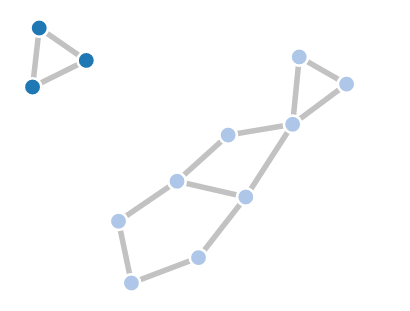
\includegraphics[width=0.3\linewidth, height=0.15\textheight]{pics/exple1.png}
\caption{The  graph has two connected components which implies $\beta_0=2$. It also has two cycles which are not boundaries
    of triangles, thus $\beta_1=2$. Higher Betti numbers are zero. }
\label{fig:prob1_6_2}
\end{minipage}
\begin{minipage}{1.0\textwidth}
\centering
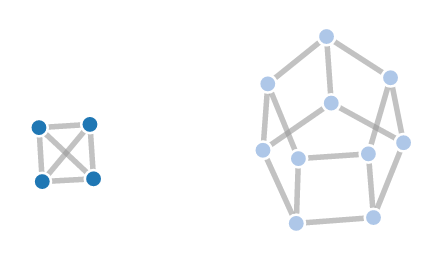
\includegraphics[width=0.4\linewidth, height=0.15\textheight]{pics/exple2.png}
\caption{The  graph has two connected components giving $\beta_0=2$. It also has 7 cycles which are not boundaries
    of triangles which yields $\beta_1=7$. Higher Betti numbers are zero here as well. If the different sides of the hexagonal prism (right component) are covered with
    triangles then we get instead $\beta_1=0$ and  $\beta_2=1$.}
\label{fig:prob1_6_1}
\end{minipage}
\end{figure}

	 
 
\newpage
~~\\
Now, lets us go back to persistent homology and make this notion a bit more precise. For that, let us reintroduce the persistent parameter $\varepsilon$ and let $K_\varepsilon$ be again an independence complex.   It is clear that  if 
$|{\sf Patients}(g)\cap{\sf Patients}(g')|\geq \varepsilon_1  $ and $ \varepsilon_1 \geq \varepsilon_2$
then the pair $(g, g')$, which is an edge in ${G}_{\varepsilon_1},$ is also is an edge in $G_{\varepsilon_2}$. This means that
${G}_{\varepsilon_1}$ is a subgraph of ${G}_{\varepsilon_2}$, thus, we have
  $K_{\varepsilon_2}\subset  K_{\varepsilon_1}$ whenever $\varepsilon_1 \geq \varepsilon_2$ (since an independent set for a given graph is also independent set for any of its subgraphs). The mapping $\varepsilon \mapsto K_\varepsilon$ is functorial.
It turns out that homology itself is  functorial  and
all  this functoriality  is the mathematical reason why the following is correct: one can track the Betti numbers over a range 
of values $\varepsilon_1 \geq \varepsilon_2 \geq \varepsilon_3\geq \cdots$ and consider the subrange where 
the Betti numbers are not changing (significantly). Pathways within this subrange are considered to have passed our test and declared robust computation.
   
 
\subsection*{Quantum computations and D-Wave quantum processor}  
Here  we will first introduce quantum computation in general and quantum annealing in particular. 
%We will also discuss D-Wave 2000Q processor which comes with 2000 qbits (quantum bits). 
We conclude this section by pinpointing to where quantum computing (precisely, our quantum algorithms  \cite{raoufHomology} and  \cite{raoufQubo}  is used within
the proposal of this paper.   

~~\\
Quantum computers use non-classical and counterintuitive features of quantum mechanics, such as superposition and tunnelling, to perform large scale calculations 
exponentially faster than classical processors. In order to exploit the capabilities of  quantum computers, the  
given problem needs to be embedded into the quantum realm, that is, represented as a quantum system. An example of that is the binary quadratic optimization problem 
\begin{equation}
	{\it argmin}_{\mathbb Z_2^n} Q(x_1,\cdots, x_n) 
\end{equation}
 which can be mapped as finding the ground state of an Ising model (a particularly interesting type of quantum systems). The binary variables in the objective functions are replaced with Pauli operators. The   values of a given variable $x_i$ are implemented as eigenstates of the corresponding Pauli operator. The superposition of the two values is called a qubit (thus, each variable introduces a qubit).  The quadratic monomials $Q_{ij}x_ix_j$ between two variables $x_i$ and $x_j$ are understood as couplings between the two corresponding operators with coupling strength~$Q_{ij}$. Quantum algorithms favour the correct value of $x_i$ by amplifying the corresponding coefficient
in the superposition.  

~~\\
Adiabatic quantum computations (AQC) \cite{farhi} are particular type of quantum algorithms which solve the ground state problem using the tunnelling feature. The quantum system, which is made time dependent by perturbing the problem Hamiltonian, 
evolves by tunnelling through the local minima to the desired solution. This is radically different from the classical thermal evolution where the system might get stuck at a local minima if the potential barrier around it is significant.  D-Wave implements AQC through a particular perturbation scheme \cite{natueDwave}. It involves a particular type of coupling (a particular configuration of the spins) and a particular evolution path (i.e., perturbation terms). From the user point of view, it suffices to enter, through a cloud based interface, the coefficients of the cost function (which will be understood as coupling and external field strengths) and gets the answer as string of binary. 

%{\color{blue} Accoding to Gordon\footnote{
%{\color{blue}
% An ME solution using a commercial quantum processor:
%The authors demonstrate solving an ME problem in cancer genomics, using their formulation and a commercial quantum processor. Here the central issue seems to be: how excited should a reader be about quantum processors for a range practical optimization problems in cancer genomics? It would be worth saying more about the processor, how it can actually be used (who can buy/use one?), and the future of such processors in cancer genomics, including increases in the scale of problem that will be addressable. For ME problems, the authors suggest that the processor should solve the problem rapidly, but they give no timing results, and give no timing results for using classical computing for solving their formulation. }
%}
%\footnote{
%\color{blue}
%Gordon: Could this also be solved by standard computing approaches, i.e. non-quantum approaches? If so, perhaps demonstrate this? And, how available are quantum solvers? 
%}
%\footnote{
%\color{blue}
%Gordon: Probably should say more about the hardware? is it available? What would be needed in order to use it? 
%}, people interest will be around this section: how it works, the hardware and how to access it}

~~\\
There are two computational bottlenecks in our proposal detailed in the previous sections. The first is
the construction of the (facets of the) simplicial complexes and the second being the homology calculation itself. 
These two computations scale exponentially with size of the input (i.e., the number of
genes in the mutation data) which makes them beyond the capabilities of classical computers and can only handled using quantum computing. 
Both questions have been discussed  in details in \cite{raoufHomology} and  \cite{raoufQubo} 
so we refrain from elaborating on them here.  

  
% \subsection*{Quantum computation of $H_*(K_\varepsilon)$ } 
%To compute  the homology  of  the persistent pathway  complex  $K_\varepsilon$
%we will use the quantum algorithm \cite{raoufNerve} (we might also use \cite{raoufHomology} but  \cite{raoufNerve} is ``optimal").   In this case, 
%$$
%	H_*(G_\varepsilon)=H_*(K_\varepsilon) = H_*(\mathcal N_\varepsilon),
%$$  
%where $\mathcal N_\varepsilon$ is the nerve of an edge clique cover of $G_\varepsilon$. The passage to the edge clique cover nerve 
%gives an exponential reduction of the size of the problem.  Indeed,  the size of the 1-skeleton of $\mathcal N_\varepsilon$  is 
%of order $O(log(n))$, with $n$ being the number of genes = vertices of $G_\varepsilon$. 
%We refer the interested reader to the paper \cite{raoufNerve} for a detailed account.
%%\section*{Co-occurence}
%%{\color{blue}	 
%%- co-occurrence = define the graph $G$ for the space of pathways: two pathways are connected if they have a least a patient in common. Co-Occurrences are the cliques of this graph. We get
%%a clique complex ! and we can do this for each patient (in addition to persitence complex)
%%}

\section*{Real mutation data}
We have applied our approach to two mutation data.  Acute myeloid leukemia \cite{doi:10.1056/NEJMoa1301689} and Glioblastoma multiform \cite{GBM2008}. For both data, we have computed the assignment tumour $\mapsto$ pathways through persistent pathway complexes (thus declared robust output).  
The complete result is presented in long tables (not included here  but can be provided upon request). 
Interestingly, our calculation also shows  that 
AML data is homotopy equivalent to a sphere while GBM data is homotopy equivalent to figure eight (genus-2 surface). 

\subsection*{AML}
%{\color{blue} Gordon: Are these extra pathways credible? }


The data has a cohort of 200 patients and 33 genes (\cite{doi:10.1056/NEJMoa1301689}). { We have chosen the coverage threshold $\eta=80$ patient. We also neglected all genes 
which have less than 6 patients.  These numbers are chosen using what one might call the persistence of persistence homology: stability of barecodes for pairs $(\varepsilon, \eta) \geq (6, 80))$ while
barecodes for pairs less than (6, 80) exhibit strong variations.  This is also consistent with the fact that choosing genes   with less than  5 or 6  patients are  not common in such studies (genes with low number of patients are not considered robust enough and are very prone to errors. It is an extra precaution
one takes which is commonly used in the field).    
Now for the numbers of patients and coverage we have chosen, the Betti numbers are computed for various values of $\varepsilon$ in the table below:
\begin{center}
\begin{tabular}{cccc}
	$\varepsilon$ &   $|\mathcal N_\varepsilon|$ &  $density(\mathcal N_\varepsilon)$  & $\beta_i$\\
	\hline\\
	                   1 &               					   6 & 								0.86	& $1, 0,0, \cdots$\\
	\hline\\
				2 &							84	& 						0.97		&	 $1, 0,0, \cdots$ \\
	\hline\\
				3 &							50	& 						1		&	 $1, 0,0, \cdots$ \\
\end{tabular}
\end{center}
Figure 3 below gives the (1-skeleton) of the nerve $\mathcal N_\varepsilon := \mathcal N(K_\varepsilon)$ for $\varepsilon=1$. The Betti numbers $\beta_i$ are not changing  thus $\varepsilon=1$ is a reasonable choice. 
Recall that each  node represents a pathway and two pathways are connected in they intersect (as sets of genes). We have used different colours to different pathways (no other meaning for the colouring). The nodes are as follows:

{\footnotesize
\begin{tabular}{l|l}
 \hline\\
 color & genes in the pathway\\
 \hline\\
 Blue &  'PML.RARA', 'MYH11.CBFB', 'RUNX1.RUNX1T1', 'TP53', 'NPM1', 'RUNX1' \\
  \hline\\
 Blue light & 'PML.RARA', 'MYH11.CBFB', 'RUNX1.RUNX1T1', 'TP53', 'NPM1', 'MLL.PTD'\\	
  \hline\\
  Orange &  'PML.RARA', 'MYH11.CBFB', 'RUNX1.RUNX1T1', 'DNMT3A'\\
   \hline\\
  Orange light & 'Other Tyr kinases', 'MYH11.CBFB', 'MLL.PTD', 'NPM1'\\
   \hline\\
      Green &  'MLL-X fusions', 'TP53', 'FLT3'\\
       \hline\\
    Green light &  'Other Tyr kinases', 'MYH11.CBFB', 'DNMT3A', 'MLL-X fusions' \\
     \hline
\end{tabular}
}

%
%     Orange= ['PML.RARA', 'MYH11.CBFB', 'RUNX1.RUNX1T1', 'DNMT3A'], Orange light=['Other Tyr kinases', 'MYH11.CBFB', 'MLL.PTD', 'NPM1'], 
%    Green=['MLL-X fusions', 'TP53', 'FLT3'], 
%    Green light=['Other Tyr kinases', 'MYH11.CBFB', 'DNMT3A', 'MLL-X fusions'],
%    Blue=['PML.RARA', 'MYH11.CBFB', 'RUNX1.RUNX1T1', 'TP53', 'NPM1', 'RUNX1'],  
%    Blue light=['PML.RARA', 'MYH11.CBFB', 'RUNX1.RUNX1T1', 'TP53', 'NPM1', 'MLL.PTD'].  
\begin{figure}[!htbp]\label{exples}
	\begin{center}
      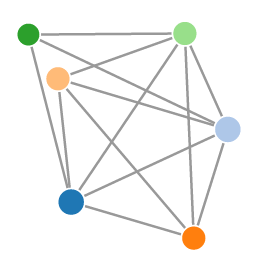
\includegraphics[scale=0.5]{pics/nerveAML.png} 
      \end{center}
    \caption{{\small The 1-skeleton of the nerve $\mathcal N_\varepsilon$ for $\varepsilon=1$ for AML data. 
    In this case, the nerve is homotopy equivalent to the sphere. The different pathways represented by the nodes are given in the table above.}
    %The pathways here have less chance
    %to be affected by the noise. 
}
\label{AMLnerve}
\end{figure}	

\subsection*{GBM}
The second mutation data is taken from \cite{GBM2008}.  It has 84 patients and around 100 genes.
Approximately, 70\% of the genes have very low coverage so we removed them from the data; precisely
we have removed all genes with less than 10 patients. We have used the complex
$K_\eta$ and we have   $\varepsilon$ fixed to 7.  Concerning the choice of these numbers, the same justification, given above, applies here. 

\begin{center}
\begin{tabular}{cccc}
	$\eta$ &   $|\mathcal N_\eta|$ &  $density(\mathcal N_\eta)$  & $\beta_i$\\
	\hline\\
				66 &							15	& 						0.73		&	 $1, 2,0, \cdots$ \\
	\hline\\
				67 &							14	& 						0.74		&	 $1, 2,0, \cdots$ \\
	\hline\\
				68 &							12	& 						0.72		&	 $1, 2,0, \cdots$ \\		
	\hline\\
				69 &							6	& 						0.6		&	 $1, 0,0, \cdots$ \\	
	\hline\\
				70 &							50	& 						1		&	 $1, 0,0, \cdots$ \\			
\end{tabular}
\end{center}
   	 
\begin{figure}[!htbp]\label{exples}
\begin{center}
      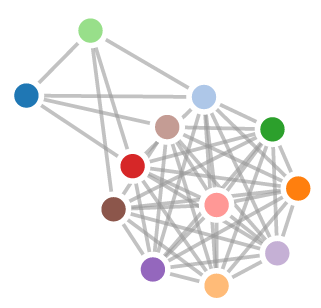
\includegraphics[scale=0.5]{pics/nerveGBM.png} 
      \end{center}
    \caption{{\small The nerve for the space of pathways for GBM data (see table below). The nerve is homotopy equivalent to a genus-2 surface.}
}
\end{figure}

~~\\
The following table provides the legend for the Figure 4 corresponding the GBM data:\\
{\footnotesize
\begin{tabular}{l|l}
  color & genes in the pathway\\
 \hline\\
 blue  & RB1,  NF1,  CYP27B1,  CDKN2B \\ \hline\\
 blue light & RB1,  NF1,  MDM2,  AVIL-CTDSP2,  CDKN2B\\\hline\\
 orange & TP53,  MDM2,  OS9,  CDKN2A\\\hline\\
 orange light & TP53,  MDM2,  AVIL-CTDSP2,  CDKN2A\\\hline\\
 green& TP53,  MDM2,  DTX3,  CDKN2A\\\hline\\
  green light & RB1,  NF1,  CDK4,  CDKN2B\\\hline\\
  brown& TP53,  CDK4,  CDKN2A\\\hline\\
  brown light& TP53,  CYP27B1,  CDKN2A\\\hline\\
   purple& TP53,  MDM2,  AVIL-CTDSP2,  MTAP\\\hline\\
   purple light & TP53,  MDM2,  DTX3,  MTAP\\\hline\\
  red& RB1,  NF1,  MDM2,  OS9,  CDKN2B\\\hline\\
   pink& TP53,  MDM2,  OS9,  MTAP\\\hline
 \end{tabular}
 } 
 
   
     
 
 

 

\section*{Conclusion}
Our goal in this paper is  the introduction of quantum computation in pathway computations and  
the proposal to use topological analysis on the space of pathways. We have demonstrated both through  real data
where have reproduced results of earlier works in addition to new findings which we hope will have some impact in the field.  
We have argued that the consideration of the pathways collectively, that is, as a topological space not only brings
all the algebraic machinery (eg., persistent homology showcased here) but also might help in
revealing novel  relations between these pathways.  Indeed, we have seen that the homology in
the case of AML  indicates that the mutation data has a shape of a sphere. However, in the case of GBM, we get a final set of pathways which has the  topology of
a double torus (or more technically a genus-2 surface). This intriguing observation raises the question of whether this fact translates into a new biological understanding about cancer which will be astonishing.  Such a question  is an example of the new type of hypotheses one can now  formulate about the data and that target 
 the connections between the pathways (global properties of the set of pathways). This might help in revealing some indications on the way  mutations work collectively in causing cancer. 

\section*{Acknowledgement}
We thank Dr. G. Robertson (BC Genome) and Dr. S. Rezaei  for  their constructive feedback and comments that greatly improved the manuscript.


%\section*{Author contributions statement}
%R. D and H.A designed the algorithms. R. D and H.A conceived the experiments and analysed the results. All authors wrote and reviewed the manuscript. 


%Must include all authors, identified by initials, for example:
%A.A. conceived the experiment(s),  A.A. and B.A. conducted the experiment(s), C.A. and D.A. analysed the results.  All authors reviewed the manuscript. 

%\section*{Additional information}

%To include, in this order: \textbf{Accession codes} (where applicable); 
%\textbf{Competing financial interests}\\ 
%The authors declare no competing financial interests.
 
 
 


 
\bibliography{c}


\end{document}
\newpage
\appendix



\section*{GBM pathways}
	 Results for GBM data: The table below reports the final pathways in Figure 4. 
	 Details on the data,  the parameters  and how the pathways are comoputed using persistent homology can be found in Section 3.2. 
\begin{center}	 
\begin{small}	 
\begin{tabular}{l|c}
	 pathway & coverage $\eta$\\
	 \hline\\
       RB1 ,  NF1 ,  CYP27B1 ,  CDKN2B   &  70\\ 
      RB1 ,  NF1 ,  MDM2 ,  AVIL-CTDSP2 ,  CDKN2B   &  69\\ 
      TP53 ,  MDM2 ,  OS9 ,  CDKN2A   &  69\\ 
      TP53 ,  MDM2 ,  AVIL-CTDSP2 ,  CDKN2A   &  69\\ 
      TP53 ,  MDM2 ,  DTX3 ,  CDKN2A   &  69\\ 
      RB1 ,  NF1 ,  CDK4 ,  CDKN2B   &  69\\ 
      RB1 ,  NF1 ,  MDM2 ,  OS9 ,  CDKN2B   &  68\\ 
      TP53 ,  MDM2 ,  OS9 ,  MTAP   &  68\\ 
      TP53 ,  MDM2 ,  AVIL-CTDSP2 ,  MTAP   &  68\\ 
      TP53 ,  MDM2 ,  DTX3 ,  MTAP   &  68\\ 
      TP53 ,  CDK4 ,  CDKN2A   &  68\\ 
      TP53 ,  CYP27B1 ,  CDKN2A   &  68\\ 
      TP53 ,  CDK4 ,  MTAP   &  67\\ 
      TP53 ,  CYP27B1 ,  MTAP   &  67\\ 
      RB1 ,  NF1 ,  CYP27B1 ,  CDKN2A   &  66\\ 
      RB1 ,  NF1 ,  MDM2 ,  OS9 ,  CDKN2A   &  65\\ 
      RB1 ,  NF1 ,  MDM2 ,  AVIL-CTDSP2 ,  CDKN2A   &  65\\ 
      RB1 ,  NF1 ,  MDM2 ,  DTX3 ,  CDKN2B   &  65\\ 
      RB1 ,  NF1 ,  CDK4 ,  CDKN2A   &  65\\ 
      RB1 ,  NF1 ,  CYP27B1 ,  MTAP   &  65\\ 
      RB1 ,  NF1 ,  MDM2 ,  OS9 ,  MTAP   &  64\\ 
      RB1 ,  NF1 ,  MDM2 ,  AVIL-CTDSP2 ,  MTAP   &  64\\ 
      RB1 ,  NF1 ,  CDK4 ,  MTAP   &  64\\ 
      RB1 ,  NF1 ,  MDM2 ,  DTX3 ,  CDKN2A   &  62\\ 
      RB1 ,  NF1 ,  MDM2 ,  DTX3 ,  MTAP   &  61\\ 
      TP53 ,  MDM2 ,  AVIL-CTDSP2 ,  SEC61G   &  60\\ 
      RB1 ,  NF1 ,  EGFR ,  OS9   &  60\\ 
      TP53 ,  MDM2 ,  OS9 ,  SEC61G   &  59\\ 
      TP53 ,  MDM2 ,  DTX3 ,  SEC61G   &  59\\ 
      PTEN ,  IFNA21 ,  MDM2 ,  AVIL-CTDSP2   &  58\\ 
      TP53 ,  MDM2 ,  AVIL-CTDSP2 ,  IFNA21   &  58\\ 
      RB1 ,  NF1 ,  EGFR ,  DTX3   &  58\\ 
      PTEN ,  IFNA21 ,  CYP27B1   &  58\\   
      PTEN ,  IFNA21 ,  MDM2 ,  OS9   &  57\\ 
      TP53 ,  MDM2 ,  OS9 ,  IFNA21   &  57\\ 
      TP53 ,  MDM2 ,  DTX3 ,  IFNA21   &  57\\ 
      PTEN ,  IFNA21 ,  CDK4   &  57\\ 
      RB1 ,  NF1 ,  MDM2 ,  AVIL-CTDSP2 ,  SEC61G   &  55\\ 
      PTEN ,  IFNA21 ,  MDM2 ,  DTX3   &  55\\ 
      TP53 ,  MDM2 ,  AVIL-CTDSP2 ,  ELAVL2   &  55\\ 
      RB1 ,  NF1 ,  MDM2 ,  OS9 ,  SEC61G   &  54\\ 
      TP53 ,  MDM2 ,  OS9 ,  ELAVL2   &  54\\ 
      TP53 ,  MDM2 ,  DTX3 ,  ELAVL2   &  54\\
      \end{tabular}
      \end{small}
      \newpage
      
      \begin{small}
      \begin{tabular}{l|c} 
      RB1 ,  NF1 ,  MDM2 ,  AVIL-CTDSP2 ,  IFNA21   &  53\\ 
      TP53 ,  CDK4 ,  IFNA21   &  53\\ 
      TP53 ,  CDK4 ,  ELAVL2   &  53\\ 
      TP53 ,  CYP27B1 ,  IFNA21   &  53\\ 
      TP53 ,  CYP27B1 ,  ELAVL2   &  53\\ 
      RB1 ,  NF1 ,  MDM2 ,  OS9 ,  IFNA21   &  52\\ 
      RB1 ,  NF1 ,  MDM2 ,  DTX3 ,  SEC61G   &  52\\ 
      RB1 ,  NF1 ,  MDM2 ,  AVIL-CTDSP2 ,  ELAVL2   &  51\\ 
      RB1 ,  NF1 ,  CYP27B1 ,  IFNA21   &  51\\ 
      RB1 ,  NF1 ,  CYP27B1 ,  ELAVL2   &  51\\ 
      RB1 ,  NF1 ,  MDM2 ,  OS9 ,  ELAVL2   &  50\\ 
      RB1 ,  NF1 ,  CDK4 ,  IFNA21   &  50\\ 
      RB1 ,  NF1 ,  CDK4 ,  ELAVL2   &  50\\ 
      RB1 ,  NF1 ,  MDM2 ,  DTX3 ,  IFNA21   &  49\\ 
      RB1 ,  NF1 ,  MDM2 ,  DTX3 ,  ELAVL2   &  47   
\end{tabular}	 
\end{small}
\end{center}


\newpage

\section*{AML pathways list}
 The following table gives the list of all 65 pathways of $\mathcal N_1$ (Figure \ref{AMLnerve})  and their coverage. 
 Details about the data and how  the pathways are obtained using persistent homology can be found in Section 3.1.  
All pathways listed below passed our robustness test.
\begin{center} 
\begin{small}
\begin{tabular}{l|c}
	pathway & coverage\\
	\hline\\
    PML.RARA ,  MYH11.CBFB ,  RUNX1.RUNX1T1 ,  TP53 ,  NPM1 ,  RUNX1   & 
  123\\  
    PML.RARA ,  MYH11.CBFB ,  RUNX1.RUNX1T1 ,  TP53 ,  NPM1 ,  MLL.PTD   & 
  113\\  
    PML.RARA ,  MYH11.CBFB ,  RUNX1.RUNX1T1 ,  DNMT3A  &  85\\  
    Other Tyr kinases ,  MYH11.CBFB ,  MLL.PTD ,  NPM1  &  83\\  
    MLL-X fusions ,  TP53 ,  FLT3  &  81\\  
    Other Tyr kinases ,  MYH11.CBFB ,  DNMT3A ,  MLL-X fusions   & 
  80\\  
    PML.RARA ,  MYH11.CBFB ,  Cohesin ,  Other modifiers  &  78\\  
    MLL-X fusions ,  DNMT3A ,  RUNX1.RUNX1T1 ,  MYH11.CBFB  &  78\\  
    PML.RARA ,  MYH11.CBFB ,  RUNX1.RUNX1T1 ,  TP53 ,  PHF6 ,  IDH1   & 
  75\\  
    Other myeloid TFs ,  MYH11.CBFB ,  Cohesin ,  Other modifiers   & 
  74\\  
    Other Tyr kinases ,  FLT3 ,  MLL-X fusions  &  74\\  
    PML.RARA ,  MYH11.CBFB ,  RUNX1.RUNX1T1 ,  TP53 ,  IDH2  &  70\\  
    PML.RARA ,  MYH11.CBFB ,  RUNX1.RUNX1T1 ,  CEBPA ,  RUNX1   & 
  66\\  
    PML.RARA ,  MYH11.CBFB ,  RUNX1.RUNX1T1 ,  TP53 ,  PHF6 ,  MLL.PTD   & 
  65\\  
    Other myeloid TFs ,  MYH11.CBFB ,  TP53 ,  RUNX1.RUNX1T1 ,  RUNX1   & 
  65\\  
    PML.RARA ,  PTPs ,  IDH2 ,  TET2  &  65\\  
    PML.RARA ,  MYH11.CBFB ,  TET2 ,  IDH2    &  64\\  
    MLL-X fusions ,  TP53 ,  RUNX1.RUNX1T1 ,  MYH11.CBFB ,  IDH2   & 
  63\\  
    PML.RARA ,  MYH11.CBFB ,  RUNX1.RUNX1T1 ,  CEBPA ,  PHF6 ,  MLL.PTD   & 
  62\\  
    PML.RARA ,  KRAS/NRAS ,  PHF6 ,  MLL.PTD ,  KIT  &  62\\  
    MLL-X fusions ,  TP53 ,  RUNX1.RUNX1T1 ,  MYH11.CBFB ,  IDH1   & 
  62\\  
    MLL-X fusions ,  TP53 ,  RUNX1.RUNX1T1 ,  MYH11.CBFB ,  RUNX1   & 
  62\\  
    Other myeloid TFs ,
    MYH11.CBFB ,
    TP53 ,
    RUNX1.RUNX1T1 ,
    PHF6 ,
    MLL.PTD   & 
  61\\  
    PML.RARA ,  KRAS/NRAS ,  PHF6 ,  MLL.PTD ,  RUNX1.RUNX1T1   & 
  61\\  
    PML.RARA ,  KIT ,  TP53 ,  IDH2  &  60\\  
    PML.RARA ,  KIT ,  TP53 ,  RUNX1  &  59\\  
    MLL-X fusions ,  TET2 ,  MYH11.CBFB ,  IDH2  &  57\\  
    PML.RARA ,  PTPs ,  IDH2 ,  KIT  &  56\\  
    PML.RARA ,  KIT ,  CEBPA ,  RUNX1  &  56\\  
    PML.RARA ,  KIT ,  TP53 ,  PHF6 ,  MLL.PTD  &  55\\  
    PML.RARA ,  PTPs ,  IDH2 ,  RUNX1.RUNX1T1  &  55\\  
    PML.RARA ,  PTPs ,  RUNX1 ,  KIT  &  55\\  
    Other myeloid TFs ,  KIT ,  TP53 ,  RUNX1  &  55\\  
    PML.RARA ,  PTPs ,  RUNX1 ,  RUNX1.RUNX1T1  &  54\\  
    MLL-X fusions ,  TP53 ,  KIT ,  IDH2  &  53\\  
    PML.RARA ,  KIT ,  CEBPA ,  PHF6 ,  MLL.PTD  &  52\\  
    MLL-X fusions ,  TP53 ,  RUNX1.RUNX1T1 ,  MYH11.CBFB ,  MLL.PTD   & 
  52\\  
    Ser-Tyr kinases ,  RUNX1.RUNX1T1 ,  PTPs ,  MLL.PTD  &  52\\  
    MLL-X fusions ,  TP53 ,  KIT ,  RUNX1  &  52\\  
    Other myeloid TFs ,  KIT ,  TP53 ,  PHF6 ,  MLL.PTD  &  51\\  
    PML.RARA ,  WT1 ,  RUNX1.RUNX1T1 ,  TP53  &  51\\  
    PML.RARA ,  MYH11.CBFB ,  TET2 ,  PHF6  &  50\\  
    PML.RARA ,  KIT ,  Cohesin  &  50\\  
    \end{tabular}
    \end{small}
  
    \begin{small}
    \begin{tabular}{l|c}
    Other Tyr kinases ,  MYH11.CBFB ,  IDH2 ,  MLL-X fusions  &  49\\  
    Other Tyr kinases ,  MYH11.CBFB ,  IDH1 ,  MLL-X fusions  &  48\\  
    Other Tyr kinases ,  MYH11.CBFB ,  MLL.PTD ,  PHF6 ,  Other myeloid TFs   & 
  47\\  
    Other Tyr kinases ,  KRAS/NRAS ,  PHF6 ,  MLL.PTD  &  47\\  
    Other myeloid TFs ,  MYH11.CBFB ,  TET2 ,  PHF6  &  46\\  
    MLL-X fusions ,  Cohesin ,  MYH11.CBFB  &  46\\  
    Other myeloid TFs ,  KIT ,  Cohesin  &  46\\  
    Other Tyr kinases ,  MYH11.CBFB ,  IDH1 ,  PHF6  &  45\\  
    PML.RARA ,  PTPs ,  MLL.PTD ,  KIT  &  45\\  
    PML.RARA ,  WT1 ,  TET2  &  45\\  
    PML.RARA ,  PTPs ,  MLL.PTD ,  RUNX1.RUNX1T1  &  44\\  
    MLL-X fusions ,  TP53 ,  RUNX1.RUNX1T1 ,  WT1  &  44\\  
    MLL-X fusions ,  Cohesin ,  KIT  &  43\\  
    MLL-X fusions ,  TP53 ,  KIT ,  MLL.PTD  &  42\\  
    Other Tyr kinases ,  PTPs ,  IDH2  &  41\\  
    Other Tyr kinases ,  MYH11.CBFB ,  MLL.PTD ,  MLL-X fusions   & 
  38\\  
    MLL-X fusions ,  TET2 ,  WT1  &  38\\  
    Spliceosome ,  CEBPA  &  37\\  
    Spliceosome ,  PTPs  &  36\\  
    Spliceosome ,  Other myeloid TFs  &  36\\  
    Other Tyr kinases ,  WT1 ,  MLL-X fusions  &  30\\  
    Other Tyr kinases ,  PTPs ,  MLL.PTD  &  30\\    
\end{tabular}
\end{small}
\end{center}


%~~\\
%\begin{tiny}
%\begin{tabular}{c|l|l}
%sample ID & pathways & cyto\\
%\hline
%0 &   0, 1, 2, 6, 8, 11, 12, 13, 15, 16, 18, 19, 23, 24, 25, 27, 28, 29, 30, 31, 33, 35, 40, 41, 42, 51, 52, 53    & Good\\
%1 &   0, 1, 2, 7, 8, 11, 12, 13, 14, 17, 18, 20, 21, 22, 23, 30, 33, 36, 37, 40, 53, 54    & Good\\
%2 &   0, 1, 2, 3, 4, 5, 6, 7, 8, 9, 10, 11, 12, 13, 14, 16, 17, 18, 19, 20, 21, 22, 23, 26, 36, 41, 43, 44, 45, 46, 47, 48, 50, 58    & Good\\
%3 &   0, 1, 2, 3, 5, 6, 7, 8, 9, 11, 12, 13, 14, 16, 17, 18, 20, 21, 22, 26, 36, 41, 43, 44, 45, 47, 48, 50, 58    & Good\\
%4 &   0, 1, 2, 3, 5, 6, 8, 10, 11, 12, 13, 15, 16, 18, 19, 23, 24, 25, 27, 28, 29, 30, 31, 33, 35, 40, 41, 42, 43, 44, 45, 46, 50, 51, 52, 53, 57, 58, 63, 64    & Good\\
%5 &   0, 1, 2, 4, 6, 8, 10, 11, 12, 13, 15, 16, 18, 19, 23, 24, 25, 27, 28, 29, 30, 31, 33, 35, 40, 41, 42, 51, 52, 53    & Good\\
%6 &   0, 1, 2, 3, 5, 6, 7, 8, 9, 11, 12, 13, 14, 15, 16, 17, 18, 20, 21, 22, 26, 27, 30, 31, 33, 36, 37, 41, 43, 44, 45, 47, 48, 50, 51, 53, 57, 58, 61, 64    & Good\\
%7 &   0, 1, 2, 3, 5, 6, 7, 8, 9, 10, 11, 12, 13, 14, 17, 18, 19, 20, 21, 22, 23, 24, 25, 27, 28, 29, 30, 31, 32, 33, 34, 35, 36, 37, 38, 39, 40, 42, 43, 44, 45, 46, 49, 50, 51, 53, 54, 55, 56, 57, 58, 60, 61, 62, 63, 64    & Good\\
%8 &   0, 1, 2, 4, 7, 8, 10, 11, 12, 13, 14, 17, 18, 20, 21, 22, 23, 30, 33, 36, 37, 40, 53, 54    & Good\\
%9 &   0, 1, 2, 6, 8, 11, 12, 13, 15, 16, 18, 19, 23, 24, 25, 27, 28, 29, 30, 31, 33, 35, 40, 41, 42, 51, 52, 53    & Good\\
%10 &   0, 1, 2, 3, 5, 6, 7, 8, 9, 11, 12, 13, 14, 16, 17, 18, 20, 21, 22, 26, 36, 41, 43, 44, 45, 47, 48, 50, 58    & Good\\
%11 &   0, 1, 2, 6, 8, 11, 12, 13, 15, 16, 18, 19, 23, 24, 25, 27, 28, 29, 30, 31, 33, 35, 40, 41, 42, 51, 52, 53, 60, 61, 62    & Good\\
%12 &   40, 52, 54, 59, 60, 61, 62, 63    & Good\\
%13 &   0, 1, 2, 3, 5, 6, 7, 8, 9, 11, 12, 13, 14, 16, 17, 18, 19, 20, 21, 22, 24, 25, 26, 27, 28, 29, 31, 32, 34, 35, 36, 38, 39, 41, 42, 43, 44, 45, 47, 48, 49, 50, 51, 55, 56, 58    & Good\\
%14 &   0, 1, 2, 4, 6, 8, 10, 11, 12, 13, 15, 16, 18, 19, 23, 24, 25, 27, 28, 29, 30, 31, 33, 35, 40, 41, 42, 51, 52, 53    & Good\\
%15 &   0, 1, 2, 6, 8, 11, 12, 13, 15, 16, 18, 19, 23, 24, 25, 27, 28, 29, 30, 31, 33, 35, 40, 41, 42, 51, 52, 53    & Good\\
%16 &   0, 1, 2, 3, 5, 6, 7, 8, 9, 10, 11, 12, 13, 14, 17, 18, 20, 21, 22, 23, 30, 33, 36, 37, 40, 42, 43, 44, 45, 46, 48, 49, 50, 53, 54, 55, 57, 58, 63, 64    & Good\\
%17 &   0, 1, 2, 4, 6, 8, 10, 11, 12, 13, 15, 16, 18, 19, 23, 24, 25, 27, 28, 29, 30, 31, 33, 35, 40, 41, 42, 51, 52, 53    & Good\\
%18 &   0, 1, 2, 3, 5, 6, 7, 8, 9, 11, 12, 13, 14, 16, 17, 18, 19, 20, 21, 22, 24, 25, 26, 27, 28, 29, 31, 32, 34, 35, 36, 37, 38, 39, 41, 42, 43, 44, 45, 47, 48, 49, 50, 51, 55, 56, 58, 60, 61, 62    & Good\\
%19 &   0, 1, 2, 6, 8, 11, 12, 13, 15, 16, 18, 19, 23, 24, 25, 27, 28, 29, 30, 31, 33, 35, 40, 41, 42, 51, 52, 53    & Good\\
%20 &   0, 1, 2, 3, 5, 6, 7, 8, 9, 11, 12, 13, 14, 16, 17, 18, 20, 21, 22, 26, 36, 41, 43, 44, 45, 47, 48, 50, 58    & Good\\
%21 &   0, 1, 2, 7, 8, 11, 12, 13, 14, 15, 16, 17, 18, 19, 20, 21, 22, 23, 24, 25, 26, 27, 28, 29, 30, 31, 32, 33, 34, 35, 36, 37, 38, 39, 40, 41, 42, 47, 49, 51, 52, 53, 54, 55, 56, 59, 60, 61, 62    & Good\\
%22 &   32, 4, 39, 9, 10, 45, 14, 47, 49, 22, 62    & Good\\
%23 &   0, 1, 2, 6, 8, 11, 12, 13, 15, 16, 18, 19, 23, 24, 25, 27, 28, 29, 30, 31, 33, 35, 40, 41, 42, 51, 52, 53    & Good\\
%24 &   0, 1, 2, 3, 4, 5, 6, 7, 8, 9, 10, 11, 12, 13, 14, 16, 17, 18, 20, 21, 22, 26, 36, 41, 43, 44, 45, 47, 48, 50, 58    & Good\\
%25 &   0, 1, 2, 3, 5, 6, 7, 8, 9, 11, 12, 13, 14, 16, 17, 18, 19, 20, 21, 22, 24, 25, 26, 27, 28, 29, 31, 32, 34, 35, 36, 38, 39, 40, 41, 42, 43, 44, 45, 47, 48, 49, 50, 51, 52, 54, 55, 56, 58, 59, 63    & Good\\
%26 &   0, 1, 2, 3, 5, 6, 7, 8, 9, 11, 12, 13, 14, 16, 17, 18, 19, 20, 21, 22, 23, 26, 36, 41, 43, 44, 45, 46, 47, 48, 50, 58    & Good\\
%27 &   0, 1, 2, 6, 8, 9, 11, 12, 13, 14, 15, 16, 18, 19, 22, 23, 24, 25, 27, 28, 29, 30, 31, 32, 33, 35, 39, 40, 41, 42, 45, 47, 49, 51, 52, 53, 62    & Good\\
%28 &   0, 1, 2, 4, 6, 8, 10, 11, 12, 13, 15, 16, 18, 19, 23, 24, 25, 27, 28, 29, 30, 31, 33, 35, 40, 41, 42, 51, 52, 53    & Good\\
%29 &   0, 1, 2, 6, 7, 8, 9, 11, 12, 13, 14, 17, 18, 20, 21, 22, 23, 30, 33, 36, 37, 40, 42, 48, 49, 53, 54, 55    & Good\\
%30 &   0, 1, 2, 4, 5, 6, 7, 8, 10, 11, 12, 13, 15, 16, 17, 18, 19, 20, 21, 23, 24, 25, 26, 27, 28, 29, 30, 31, 33, 34, 35, 36, 38, 40, 41, 42, 43, 44, 48, 51, 52, 53, 54, 55, 56, 58, 59, 63    & Good\\
%31 &   37    & Good\\
%32 &   0, 1, 2, 3, 5, 6, 7, 8, 9, 11, 12, 13, 14, 16, 17, 18, 20, 21, 22, 26, 36, 41, 43, 44, 45, 47, 48, 50, 58    & Good\\
%33 &   0, 1, 2, 3, 5, 6, 8, 10, 11, 12, 13, 15, 16, 18, 19, 23, 24, 25, 27, 28, 29, 30, 31, 33, 35, 40, 41, 42, 43, 44, 45, 46, 50, 51, 52, 53, 57, 58, 63, 64    & Good\\
%34 &   0, 1, 2, 6, 7, 8, 9, 11, 12, 13, 14, 17, 18, 20, 21, 22, 23, 30, 33, 36, 37, 40, 42, 48, 49, 53, 54, 55    & Good\\
%35 &   0, 1, 2, 4, 6, 8, 10, 11, 12, 13, 15, 16, 18, 19, 23, 24, 25, 27, 28, 29, 30, 31, 33, 35, 40, 41, 42, 51, 52, 53    & Good\\
%36 (last good) &   10, 4    & Good\\
%37 &   0, 1, 2, 3, 5, 7, 8, 64, 44, 61, 15, 50, 51, 20, 53, 57, 33, 27, 37, 30, 31    & Intermediate\\
%38 &   35, 6, 39, 8, 41, 13, 46, 45, 50, 18, 19, 9, 22, 23, 47, 29    & Intermediate\\
%39 &   0, 32, 34, 43, 38, 33, 11, 12, 14, 15, 16, 17, 21, 25, 24, 57, 26, 27, 28, 30, 31    & Intermediate\\
%40 &   0, 11, 12, 14, 15, 16, 17, 21, 24, 25, 26, 27, 28, 30, 31, 32, 33, 34, 37, 38, 43, 57    & Intermediate\\
%41 &   35, 60, 12, 46, 18, 19, 23, 28    & Intermediate\\
%42 &   0, 1, 2, 3, 5, 7    & Intermediate\\
%43 &   0, 1, 2, 3, 4, 5, 6, 7, 9, 10, 48, 49, 55, 42    & Intermediate\\
%44 &   0, 6, 9, 12, 14, 15, 16, 19, 21, 23, 25, 26, 28, 31, 32, 33, 38, 41, 42, 46, 47, 48, 49, 52, 55, 59, 60, 61, 62    & Intermediate\\
%45 &   0, 1, 10, 3, 4    & Intermediate\\
%46 &   2, 43, 5, 7, 11, 34, 46, 15, 16, 17, 19, 23, 24, 57, 26, 27, 30, 37    & Intermediate\\
%47 &   10, 4    & Intermediate\\
%48 &   0, 1, 3, 4, 6, 9, 10, 15, 27, 30, 31, 33, 37, 42, 48, 49, 51, 53, 55, 57, 61, 64    & Intermediate\\
%49 &   0, 1, 2, 3, 4, 5, 7, 10    & Intermediate\\
%50 &   0, 1, 2, 3, 4, 5, 7, 41, 10, 15, 16, 59, 52, 26, 47    & Intermediate\\
%51 &   0, 1, 3, 4, 6, 9, 10, 15, 27, 30, 31, 33, 37, 42, 48, 49, 51, 53, 55, 57, 61, 64    & Intermediate\\
%52 &   0, 1, 3, 37, 6, 33, 64, 9, 42, 15, 48, 49, 51, 53, 55, 57, 27, 61, 30, 31    & Intermediate\\
%53 &   2, 59, 5, 7, 41, 15, 16, 52, 26, 47    & Intermediate\\
%54 &   0, 1, 2, 3, 4, 5, 7, 10, 46, 19, 23    & Intermediate\\
%55 &   0, 1, 2, 3, 4, 5, 6, 7, 9, 10, 48, 49, 55, 42    & Intermediate\\
%56 &   0, 1, 2, 3, 4, 5, 7, 10    & Intermediate\\
%57 &   1, 3, 8, 13, 18, 19, 20, 22, 23, 29, 35, 36, 37, 39, 44, 45, 46, 50, 51, 53, 56, 58, 64    & Intermediate\\
%58 &   0, 2, 5, 6, 7, 8, 9, 12, 13, 14, 18, 19, 21, 22, 23, 25, 28, 29, 31, 32, 33, 35, 37, 38, 39, 41, 42, 45, 46, 47, 48, 49, 50, 55, 60, 61, 62    & Intermediate\\
%59 &   2, 5, 7, 46, 19, 23, 60, 61, 62    & Intermediate\\
%60 &   0, 1, 3, 4, 6, 9, 10, 48, 49, 55, 42    & Intermediate\\
%61 &   0, 1, 3, 4, 6, 40, 9, 10, 48, 49, 52, 54, 55, 59, 42, 63    & Intermediate\\
%62 &   10, 4    & Intermediate\\
%63 &   28, 18, 35, 12, 60    & Intermediate\\
%64 &   0, 8, 11, 12, 14, 15, 16, 17, 20, 21, 24, 25, 26, 27, 28, 30, 31, 32, 33, 34, 38, 43, 44, 50, 57, 60, 61, 62    & Intermediate\\
%65 &   48, 2, 59, 5, 6, 7, 8, 41, 42, 55, 44, 15, 16, 49, 50, 52, 9, 20, 26, 47    & Intermediate\\
%66 &   32, 2, 5, 7, 9, 39, 45, 14, 47, 49, 22, 62    & Intermediate\\
%67 &   0, 1, 2, 3, 5, 6, 7, 9, 42, 48, 49, 55    & Intermediate\\
%68 &   0, 1, 2, 3, 4, 5, 7, 10    & Intermediate\\
%69 &   0, 1, 2, 3, 5, 6, 7, 40, 9, 44, 8, 50, 52, 54, 20, 59, 63    & Intermediate\\
%70 &   0, 1, 34, 3, 11, 46, 15, 16, 17, 19, 43, 23, 24, 57, 26, 27, 30    & Intermediate\\
%71 &   32, 39, 9, 45, 14, 47, 49, 22, 62    & Intermediate\\
%72 &   0, 1, 34, 3, 4, 10, 11, 15, 16, 17, 43, 24, 57, 26, 27, 30    & Intermediate\\
%73 &   0, 1, 3, 8, 44, 50, 20    & Intermediate\\
%74 &   0, 1, 3, 4, 41, 10, 15, 16, 59, 52, 26, 47    & Intermediate\\
%75 &   35, 4, 60, 10, 12, 18, 28    & Intermediate\\
%76 &   0, 1, 2, 3, 4, 5, 7, 10    & Intermediate\\
%77 &   1, 2, 3, 4, 5, 6, 7, 9, 10, 13, 15, 16, 18, 19, 22, 23, 26, 29, 35, 36, 37, 39, 41, 45, 46, 47, 51, 52, 53, 56, 58, 59, 64    & Intermediate\\
%78 &   10, 4    & Intermediate\\
%79 &   2, 5, 7    & Intermediate\\
%80 &   0, 1, 2, 3, 4, 5, 7, 9, 10, 39, 45, 14, 47, 49, 32, 22, 62    & Intermediate\\
%81 &   34, 4, 5, 38, 7, 10, 43, 44, 48, 17, 20, 21, 54, 55, 56, 36, 26, 59, 58, 63    & Intermediate\\
%82 &   4, 6, 8, 9, 10, 44, 50, 20    & Intermediate\\
%83 &   2, 5, 7, 9, 14, 15, 22, 27, 30, 31, 32, 33, 37, 39, 45, 47, 49, 51, 53, 57, 61, 62, 64    & Intermediate\\
%84 &   0, 1, 3, 4, 10, 12, 13, 14, 18, 19, 21, 22, 23, 25, 28, 29, 31, 32, 33, 35, 36, 37, 38, 39, 40, 45, 46, 51, 52, 53, 54, 56, 58, 59, 63, 64    & Intermediate\\
%85 &   9, 10, 4, 6    & Intermediate\\
%86 &   0, 1, 3    & Intermediate\\
%87 &   0, 1, 10, 3, 4    & Intermediate\\
%88 &   34, 43, 37, 11, 15, 16, 17, 62, 24, 57, 26, 27, 60, 61, 30    & Intermediate\\
%89 &   0, 1, 3    & Intermediate\\
%\end{tabular}
%\end{tiny}

%\begin{tiny}
%\begin{tabular}{c|l|l}
%90 &   0, 1, 2, 3, 5, 7, 8, 64, 44, 61, 15, 50, 51, 20, 53, 57, 33, 27, 37, 30, 31    & Intermediate\\
%91 &   0, 1, 2, 3, 5, 6, 7, 9, 12, 15, 18, 19, 23, 27, 28, 30, 31, 33, 35, 37, 40, 42, 46, 48, 49, 51, 52, 53, 54, 55, 57, 59, 60, 61, 63, 64    & Intermediate\\
%92 &   0, 32, 34, 43, 38, 33, 11, 12, 14, 15, 16, 17, 21, 25, 24, 57, 26, 27, 28, 30, 31    & Intermediate\\
%93 &   59, 37, 41, 47, 16, 52, 26, 15, 60, 61, 62    & Intermediate\\
%94 &   0, 1, 2, 3, 4, 5, 7, 8, 9, 10, 39, 44, 45, 14, 47, 49, 50, 20, 32, 22, 62    & Intermediate\\
%95 &   0, 1, 2, 3, 5, 6, 7, 9, 42, 55, 46, 48, 49, 19, 23    & Intermediate\\
%96 &   0, 32, 38, 33, 12, 14, 21, 25, 28, 31    & Intermediate\\
%97 &   59, 41, 46, 47, 16, 19, 52, 23, 26, 15    & Intermediate\\
%98 &   0, 1, 10, 3, 4    & Intermediate\\
%99 &   0, 1, 3, 37, 8, 44, 50, 20    & Intermediate\\
%100 &   0, 1, 2, 4, 5, 7, 8, 11, 13, 14, 17, 20, 21, 22, 24, 25, 29, 32, 34, 36, 37, 38, 39, 40, 54, 56    & Intermediate\\
%101 &   28, 18, 35, 12, 60    & Intermediate\\
%102 &   0, 1, 3, 8, 44, 50, 20    & Intermediate\\
%103 &   0, 32, 38, 33, 12, 14, 21, 25, 28, 31    & Intermediate\\
%104 &   34, 4, 5, 38, 7, 10, 43, 44, 48, 17, 20, 21, 54, 55, 56, 36, 26, 59, 58, 63    & Intermediate\\
%105 &   32, 51, 34, 35, 38, 39, 60, 42, 61, 49, 19, 56, 55, 24, 25, 27, 28, 29, 62, 31    & Intermediate\\
%106 &   0, 1, 34, 3, 37, 11, 15, 16, 17, 43, 24, 57, 26, 27, 30    & Intermediate\\
%107 &   0, 3, 5, 10, 12, 14, 21, 25, 28, 31, 32, 33, 38, 43, 44, 45, 46, 50, 57, 58, 63, 64    & Intermediate\\
%108 &   4, 5, 6, 7, 9, 10, 12, 17, 18, 20, 21, 26, 28, 34, 35, 36, 38, 43, 44, 48, 54, 55, 56, 58, 59, 60, 63    & Intermediate\\
%109 &   3, 5, 10, 12, 15, 16, 18, 26, 28, 35, 41, 43, 44, 45, 46, 47, 50, 52, 57, 58, 59, 60, 63, 64    & Intermediate\\
%110 &   4, 40, 10, 52, 54, 59, 63    & Intermediate\\
%111 &   0, 1, 2, 3, 4, 5, 7, 10    & Intermediate\\
%112 &   0, 1, 3, 4, 5, 6, 7, 9, 10, 17, 19, 20, 21, 23, 26, 34, 36, 38, 43, 44, 46, 48, 54, 55, 56, 58, 59, 63    & Intermediate\\
%113 &   0, 1, 3    & Intermediate\\
%114 &   0, 1, 3, 12, 13, 14, 18, 19, 21, 22, 23, 25, 28, 29, 31, 32, 33, 35, 36, 37, 38, 39, 45, 46, 51, 53, 56, 58, 60, 61, 62, 64    & Intermediate\\
%115 &   0, 1, 2, 3, 5, 7, 46, 19, 23    & Intermediate\\
%116 &   1, 2, 3, 4, 5, 7, 10, 11, 13, 15, 16, 17, 18, 19, 22, 23, 24, 26, 27, 29, 30, 34, 35, 36, 37, 39, 43, 45, 46, 51, 53, 56, 57, 58, 64    & Intermediate\\
%117 &   2, 4, 37, 6, 7, 9, 10, 61, 48, 49, 55, 60, 42, 62, 5    & Intermediate\\
%118 &   0, 1, 2, 3, 5, 7    & Intermediate\\
%119 &   0, 1, 3, 40, 52, 54, 59, 60, 61, 62, 63    & Intermediate\\
%120 &   0, 32, 34, 43, 38, 33, 11, 12, 14, 15, 16, 17, 21, 25, 24, 57, 26, 27, 28, 30, 31    & Intermediate\\
%121 &   34, 4, 37, 38, 7, 63, 10, 43, 44, 48, 17, 20, 21, 54, 55, 56, 36, 26, 59, 58, 5    & Intermediate\\
%122 &   0, 1, 3, 4, 8, 10, 13, 18, 19, 22, 23, 29, 35, 39, 40, 41, 45, 46, 47, 50, 52, 54, 59, 63    & Intermediate\\
%123 &   0, 1, 2, 3, 4, 5, 6, 7, 9, 10, 48, 49, 55, 42    & Intermediate\\
%124 &   0, 1, 3, 8, 44, 46, 50, 19, 20, 23    & Intermediate\\
%125 &   48, 59, 4, 6, 41, 10, 55, 47, 16, 49, 52, 9, 26, 15, 42    & Intermediate\\
%126 &   0, 1, 2, 3, 4, 5, 7, 10    & Intermediate\\
%127 &   1, 2, 3, 5, 6, 7, 9, 13, 18, 19, 22, 23, 29, 35, 36, 37, 39, 42, 45, 46, 48, 49, 51, 53, 55, 56, 58, 64    & Intermediate\\
%128 &   0, 32, 38, 33, 12, 14, 21, 25, 28, 31    & Intermediate\\
%129 &   1, 3, 6, 9, 13, 15, 16, 18, 19, 22, 23, 26, 29, 35, 36, 37, 39, 41, 42, 45, 46, 47, 48, 49, 51, 52, 53, 55, 56, 58, 59, 64    & Intermediate\\
%130 &   28, 18, 35, 12, 60    & Intermediate\\
%131 &   2, 43, 5, 6, 7, 9, 11, 34, 15, 16, 17, 24, 57, 26, 27, 30    & Intermediate\\
%133 &   0, 1, 2, 3, 4, 5, 7, 10    & Intermediate\\
%134 &   0, 6, 8, 9, 12, 13, 14, 18, 19, 21, 22, 23, 25, 28, 29, 31, 32, 33, 35, 38, 39, 40, 41, 45, 46, 47, 50, 52, 54, 59, 63    & Intermediate\\
%135 &   32, 2, 35, 5, 7, 60, 39, 12, 45, 14, 47, 49, 18, 22, 9, 28, 62    & Intermediate\\
%136 &   3, 5, 6, 9, 10, 15, 16, 26, 37, 41, 43, 44, 45, 46, 47, 50, 52, 57, 58, 59, 63, 64    & Intermediate\\
%137 &   4, 5, 7, 9, 10, 14, 17, 19, 20, 21, 22, 23, 26, 32, 34, 36, 38, 39, 43, 44, 45, 46, 47, 48, 49, 54, 55, 56, 58, 59, 62, 63    & Intermediate\\
%138 &   1, 3, 11, 13, 15, 16, 17, 18, 19, 22, 23, 24, 26, 27, 29, 30, 34, 35, 36, 37, 39, 43, 45, 46, 51, 53, 56, 57, 58, 64    & Intermediate\\
%140 &   0, 1, 2, 3, 4, 5, 6, 7, 9, 10, 15, 27, 30, 31, 33, 37, 42, 48, 49, 51, 53, 55, 57, 61, 64    & Intermediate\\
%141 &   0, 1, 2, 3, 5, 6, 7, 9, 60, 61, 62    & Intermediate\\
%142 &   0, 32, 38, 33, 12, 14, 21, 25, 28, 31    & Intermediate\\
%143 &   0, 1, 2, 6, 8, 11, 12, 13, 15, 16, 18, 19, 23, 24, 25, 27, 28, 29, 30, 31, 33, 35, 37, 40, 41, 42, 51, 52, 53    & Intermediate\\
%144 &   0, 6, 8, 9, 11, 12, 13, 14, 15, 16, 17, 18, 19, 21, 22, 23, 24, 25, 26, 27, 28, 29, 30, 31, 32, 33, 34, 35, 38, 39, 41, 43, 45, 46, 47, 50, 57    & Intermediate\\
%145 &   2, 43, 5, 7, 11, 34, 46, 15, 16, 17, 19, 23, 24, 57, 26, 27, 30    & Intermediate\\
%146 &   0, 1, 3, 4, 6, 60, 10, 55, 12, 48, 49, 18, 35, 9, 28, 42    & Intermediate\\
%147 &   0, 32, 59, 37, 38, 33, 31, 41, 12, 46, 47, 16, 19, 52, 14, 23, 25, 26, 15, 28, 21    & Intermediate\\
%148 &   0, 1, 3    & Intermediate\\
%149 &   37    & Intermediate\\
%150 &   1, 3, 11, 13, 15, 16, 17, 18, 19, 22, 23, 24, 26, 27, 29, 30, 34, 35, 36, 37, 39, 43, 45, 46, 51, 53, 56, 57, 58, 64    & Intermediate\\
%151 (last intermediate) &   2, 5, 7, 8, 44, 50, 20    & Intermediate\\
%152 &   0, 1, 34, 3, 11, 15, 16, 17, 43, 24, 57, 26, 27, 30    & N.D.\\
%153 &   0, 1, 3, 4, 5, 8, 10, 11, 13, 14, 17, 20, 21, 22, 24, 25, 29, 32, 34, 36, 38, 39, 40, 43, 44, 45, 46, 50, 54, 56, 57, 58, 63, 64    & N.D.\\
%154 &   0, 1, 2, 3, 4, 5, 6, 7, 9, 10, 60, 61, 62    & N.D.\\
%155 &   0, 6, 9, 11, 12, 14, 15, 16, 17, 21, 24, 25, 26, 27, 28, 30, 31, 32, 33, 34, 38, 42, 43, 48, 49, 55, 57    & N.D.\\
%157 &   0, 1, 2, 4, 5, 6, 7, 8, 9, 11, 13, 14, 15, 16, 17, 20, 21, 22, 24, 25, 26, 29, 32, 34, 36, 37, 38, 39, 40, 41, 42, 47, 48, 49, 52, 54, 55, 56, 59    & Poor\\
%158 &   9, 10, 4, 6    & Poor\\
%159 &   0, 1, 4, 8, 11, 13, 14, 17, 20, 21, 22, 24, 25, 29, 32, 34, 36, 38, 39, 40, 54, 56, 60, 61, 62    & Poor\\
%160 &   0, 1, 4, 8, 11, 13, 14, 17, 20, 21, 22, 24, 25, 29, 32, 34, 36, 38, 39, 40, 54, 56    & Poor\\
%161 &   10, 4    & Poor\\
%162 &   0, 1, 3, 4, 37, 10    & Poor\\
%163 &   32, 39, 9, 45, 14, 47, 49, 22, 62    & Poor\\
%164 &   9, 11, 12, 14, 15, 16, 17, 18, 22, 24, 26, 27, 28, 30, 32, 34, 35, 37, 39, 40, 43, 45, 47, 49, 52, 54, 57, 59, 60, 62, 63    & Poor\\
%165 &   37    & Poor\\
%166 &   0, 1, 4, 6, 8, 9, 11, 13, 14, 17, 20, 21, 22, 24, 25, 29, 32, 34, 36, 38, 39, 40, 54, 56    & Poor\\
%167 &   19, 46, 23    & Poor\\
%168 &   59, 37, 6, 41, 47, 16, 52, 9, 26, 15    & Poor\\
%169 &   9, 6    & Poor\\
%170 &   0, 1, 4, 8, 11, 13, 14, 15, 17, 20, 21, 22, 24, 25, 27, 29, 30, 31, 32, 33, 34, 36, 37, 38, 39, 40, 51, 53, 54, 56, 57, 61, 64    & Poor\\
%171 &   60, 37, 62, 61    & Poor\\
%172 &   10, 4    & Poor\\
%174 &   46, 19, 23, 60, 61, 62    & Poor\\
%175 &   0, 1, 4, 8, 11, 13, 14, 17, 19, 20, 21, 22, 23, 24, 25, 29, 32, 34, 36, 38, 39, 40, 46, 54, 56    & Poor\\
%176 &   0, 1, 4, 6, 8, 9, 11, 13, 14, 15, 17, 20, 21, 22, 24, 25, 27, 29, 30, 31, 32, 33, 34, 36, 37, 38, 39, 40, 51, 53, 54, 56, 57, 61, 64    & Poor\\
%177 &   2, 5, 7, 8, 44, 46, 50, 19, 20, 23    & Poor\\
%178 &   4, 6, 40, 9, 10, 61, 48, 49, 52, 54, 55, 59, 60, 42, 62, 63    & Poor\\
%179 &   2, 5, 7, 9, 11, 14, 15, 16, 17, 22, 24, 26, 27, 30, 32, 34, 39, 43, 45, 47, 49, 57, 62    & Poor\\
%180 &   2, 59, 4, 5, 7, 8, 41, 10, 44, 15, 16, 50, 52, 20, 26, 47    & Poor\\
%181 &   60, 61, 62    & Poor\\
%183 &   4, 5, 7, 10, 17, 20, 21, 26, 34, 36, 37, 38, 43, 44, 48, 54, 55, 56, 58, 59, 60, 61, 62, 63    & Poor\\
%184 &   0, 1, 2, 3, 4, 5, 7, 8, 10, 19, 20, 24, 25, 27, 28, 29, 31, 32, 34, 35, 38, 39, 42, 44, 49, 50, 51, 55, 56    & Poor\\
%186 &   0, 1, 4, 6, 8, 9, 11, 13, 14, 17, 20, 21, 22, 24, 25, 29, 32, 34, 36, 38, 39, 40, 54, 56    & Poor\\
%187 &   0, 32, 2, 6, 5, 38, 7, 8, 12, 44, 14, 50, 20, 21, 9, 25, 33, 28, 31    & Poor\\
%188 &   32, 51, 34, 35, 6, 38, 39, 9, 42, 49, 19, 56, 55, 24, 25, 27, 28, 29, 31    & Poor\\
%189 &   0, 1, 4, 8, 11, 13, 14, 17, 20, 21, 22, 24, 25, 29, 32, 34, 36, 38, 39, 40, 54, 56    & Poor\\
%190 &   0, 1, 3, 4, 5, 8, 10, 11, 13, 14, 17, 20, 21, 22, 24, 25, 29, 32, 34, 36, 38, 39, 40, 43, 44, 45, 46, 50, 54, 56, 57, 58, 63, 64    & Poor\\
%191 &   0, 1, 4, 8, 11, 12, 13, 14, 17, 18, 19, 20, 21, 22, 23, 24, 25, 28, 29, 32, 34, 35, 36, 38, 39, 40, 46, 54, 56, 60    & Poor\\
%192 &   4, 5, 7, 8, 10, 13, 15, 17, 18, 19, 20, 21, 22, 23, 26, 27, 29, 30, 31, 33, 34, 35, 36, 37, 38, 39, 41, 43, 44, 45, 46, 47, 48, 50, 51, 53, 54, 55, 56, 57, 58, 59, 61, 63, 64    & Poor\\
%194 &   0, 1, 4, 6, 8, 9, 11, 13, 14, 17, 20, 21, 22, 24, 25, 29, 32, 34, 36, 38, 39, 40, 54, 56    & Poor\\
%195 &   0, 1, 4, 8, 11, 13, 14, 17, 20, 21, 22, 24, 25, 29, 32, 34, 36, 38, 39, 40, 54, 56    & Poor\\
%196 &   0, 1, 2, 3, 5, 6, 7, 9, 46, 19, 23, 60, 61, 62    & Poor\\
%197 &   2, 35, 5, 6, 7, 8, 12, 44, 18, 60, 50, 20, 9, 28    & Poor\\
%198 &   0, 1, 4, 8, 11, 13, 14, 17, 20, 21, 22, 24, 25, 29, 32, 34, 36, 37, 38, 39, 40, 54, 56    & Poor\\
%199 &   8, 44, 50, 20    & Poor
%\end{tabular}
%\end{tiny}

\newpage
~~\\
{The following long table gives the assignment tumour $\mapsto$ list of pathways for the AML data.}
For each tumour we assign a robust set of pathways. More specifically, for a tumour (sample ID) i the second column  gives
the list of all pathways (for sample ID i affected by mutations) which have passed our robustness test. %\afterpage 

\medskip

~~\\
%\afterpage
\scalebox{.9}{
   % \clearpage% Flush earlier floats (otherwise order might not be correct)
    %\thispagestyle{empty}% empty page style (?)
   % \begin{landscape}% Landscape page
        \centering % Center table
\begin{tiny}
\begin{tabular}{l|l|l}
sample ID & pathways & cyto\\
\hline
0 &   0, 1, 2, 6, 8, 11, 12, 13, 15, 16, 18, 19, 23, 24, 25, 27, 28, 29, 30, 31, 33, 35, 40, 41, 42, 51, 52, 53    & Good\\
1 &   0, 1, 2, 7, 8, 11, 12, 13, 14, 17, 18, 20, 21, 22, 23, 30, 33, 36, 37, 40, 53, 54    & Good\\
2 &   0, 1, 2, 3, 4, 5, 6, 7, 8, 9, 10, 11, 12, 13, 14, 16, 17, 18, 19, 20, 21, 22, 23, 26, 36, 41, 43, 44, 45, 46, 47, 48, 50, 58    & Good\\
3 &   0, 1, 2, 3, 5, 6, 7, 8, 9, 11, 12, 13, 14, 16, 17, 18, 20, 21, 22, 26, 36, 41, 43, 44, 45, 47, 48, 50, 58    & Good\\
4 &   0, 1, 2, 3, 5, 6, 8, 10, 11, 12, 13, 15, 16, 18, 19, 23, 24, 25, 27, 28, 29, 30, 31, 33, 35, 40, 41, 42, 43, 44, 45, 46, 50, 51, 52, 53, 57, 58, 63, 64    & Good\\
5 &   0, 1, 2, 4, 6, 8, 10, 11, 12, 13, 15, 16, 18, 19, 23, 24, 25, 27, 28, 29, 30, 31, 33, 35, 40, 41, 42, 51, 52, 53    & Good\\
6 &   0, 1, 2, 3, 5, 6, 7, 8, 9, 11, 12, 13, 14, 15, 16, 17, 18, 20, 21, 22, 26, 27, 30, 31, 33, 36, 37, 41, 43, 44, 45, 47, 48, 50, 51, 53, 57, 58, 61, 64    & Good\\
7 &   0, 1, 2, 3, 5, 6, 7, 8, 9, 10, 11, 12, 13, 14, 17, 18, 19, 20, 21, 22, 23, 24, 25, 27, 28, 29, 30, 31, 32, 33, 34, 35, 36, 37, 38, 39, 40, 42, 43, 44, 45, \\
& 46, 49, 50, 51, 53, 54, 55, 56, 57, 58, 60, 61, 62, 63, 64    & Good\\
8 &   0, 1, 2, 4, 7, 8, 10, 11, 12, 13, 14, 17, 18, 20, 21, 22, 23, 30, 33, 36, 37, 40, 53, 54    & Good\\
9 &   0, 1, 2, 6, 8, 11, 12, 13, 15, 16, 18, 19, 23, 24, 25, 27, 28, 29, 30, 31, 33, 35, 40, 41, 42, 51, 52, 53    & Good\\
10 &   0, 1, 2, 3, 5, 6, 7, 8, 9, 11, 12, 13, 14, 16, 17, 18, 20, 21, 22, 26, 36, 41, 43, 44, 45, 47, 48, 50, 58    & Good\\
11 &   0, 1, 2, 6, 8, 11, 12, 13, 15, 16, 18, 19, 23, 24, 25, 27, 28, 29, 30, 31, 33, 35, 40, 41, 42, 51, 52, 53, 60, 61, 62    & Good\\
12 &   40, 52, 54, 59, 60, 61, 62, 63    & Good\\
13 &   0, 1, 2, 3, 5, 6, 7, 8, 9, 11, 12, 13, 14, 16, 17, 18, 19, 20, 21, 22, 24, 25, 26, 27, 28, 29, 31, 32, 34, 35, 36, 38, 39, 41, 42, 43, 44, 45, 47, 48, 49, \\
& 50, 51, 55, 56, 58    & Good\\
14 &   0, 1, 2, 4, 6, 8, 10, 11, 12, 13, 15, 16, 18, 19, 23, 24, 25, 27, 28, 29, 30, 31, 33, 35, 40, 41, 42, 51, 52, 53    & Good\\
15 &   0, 1, 2, 6, 8, 11, 12, 13, 15, 16, 18, 19, 23, 24, 25, 27, 28, 29, 30, 31, 33, 35, 40, 41, 42, 51, 52, 53    & Good\\
16 &   0, 1, 2, 3, 5, 6, 7, 8, 9, 10, 11, 12, 13, 14, 17, 18, 20, 21, 22, 23, 30, 33, 36, 37, 40, 42, 43, 44, 45, 46, 48, 49, 50, 53, 54, 55, 57, 58, 63, 64    & Good\\
17 &   0, 1, 2, 4, 6, 8, 10, 11, 12, 13, 15, 16, 18, 19, 23, 24, 25, 27, 28, 29, 30, 31, 33, 35, 40, 41, 42, 51, 52, 53    & Good\\
18 &   0, 1, 2, 3, 5, 6, 7, 8, 9, 11, 12, 13, 14, 16, 17, 18, 19, 20, 21, 22, 24, 25, 26, 27, 28, 29, 31, 32, 34, 35, 36, 37, 38, 39, 41, 42, 43, 44, 45, 47, 48, \\
& 49, 50, 51, 55, 56, \\
& 58, 60, 61, 62    & Good\\
19 &   0, 1, 2, 6, 8, 11, 12, 13, 15, 16, 18, 19, 23, 24, 25, 27, 28, 29, 30, 31, 33, 35, 40, 41, 42, 51, 52, 53    & Good\\
20 &   0, 1, 2, 3, 5, 6, 7, 8, 9, 11, 12, 13, 14, 16, 17, 18, 20, 21, 22, 26, 36, 41, 43, 44, 45, 47, 48, 50, 58    & Good\\
21 &   0, 1, 2, 7, 8, 11, 12, 13, 14, 15, 16, 17, 18, 19, 20, 21, 22, 23, 24, 25, 26, 27, 28, 29, 30, 31, 32, 33, 34, 35, 36, 37, 38, 39, 40, 41, 42, 47, 49,\\
&  51, 52, 53, 54, 55, 56,  59, 60, 61, 62    & Good\\
22 &   32, 4, 39, 9, 10, 45, 14, 47, 49, 22, 62    & Good\\
23 &   0, 1, 2, 6, 8, 11, 12, 13, 15, 16, 18, 19, 23, 24, 25, 27, 28, 29, 30, 31, 33, 35, 40, 41, 42, 51, 52, 53    & Good\\
24 &   0, 1, 2, 3, 4, 5, 6, 7, 8, 9, 10, 11, 12, 13, 14, 16, 17, 18, 20, 21, 22, 26, 36, 41, 43, 44, 45, 47, 48, 50, 58    & Good\\
25 &   0, 1, 2, 3, 5, 6, 7, 8, 9, 11, 12, 13, 14, 16, 17, 18, 19, 20, 21, 22, 24, 25, 26, 27, 28, 29, 31, 32, 34, 35, 36, 38, 39, 40, 41, 42, 43, 44, 45, 47, 48, \\
& 49, 50, 51, 52, 54, 55, 56,  58, 59, 63    & Good\\
26 &   0, 1, 2, 3, 5, 6, 7, 8, 9, 11, 12, 13, 14, 16, 17, 18, 19, 20, 21, 22, 23, 26, 36, 41, 43, 44, 45, 46, 47, 48, 50, 58    & Good\\
27 &   0, 1, 2, 6, 8, 9, 11, 12, 13, 14, 15, 16, 18, 19, 22, 23, 24, 25, 27, 28, 29, 30, 31, 32, 33, 35, 39, 40, 41, 42, 45, 47, 49, 51, 52, 53, 62    & Good\\
28 &   0, 1, 2, 4, 6, 8, 10, 11, 12, 13, 15, 16, 18, 19, 23, 24, 25, 27, 28, 29, 30, 31, 33, 35, 40, 41, 42, 51, 52, 53    & Good\\
29 &   0, 1, 2, 6, 7, 8, 9, 11, 12, 13, 14, 17, 18, 20, 21, 22, 23, 30, 33, 36, 37, 40, 42, 48, 49, 53, 54, 55    & Good\\
30 &   0, 1, 2, 4, 5, 6, 7, 8, 10, 11, 12, 13, 15, 16, 17, 18, 19, 20, 21, 23, 24, 25, 26, 27, 28, 29, 30, 31, 33, 34, 35, 36, 38, 40, 41, 42, 43, 44, 48,\\
& 51, 52, 53, 54, 55, 56, 58, 59, 63    & Good\\
31 &   37    & Good\\
32 &   0, 1, 2, 3, 5, 6, 7, 8, 9, 11, 12, 13, 14, 16, 17, 18, 20, 21, 22, 26, 36, 41, 43, 44, 45, 47, 48, 50, 58    & Good\\
33 &   0, 1, 2, 3, 5, 6, 8, 10, 11, 12, 13, 15, 16, 18, 19, 23, 24, 25, 27, 28, 29, 30, 31, 33, 35, 40, 41, 42, 43, 44, 45, 46, 50, 51, 52, 53, 57, 58, 63, 64    & Good\\
34 &   0, 1, 2, 6, 7, 8, 9, 11, 12, 13, 14, 17, 18, 20, 21, 22, 23, 30, 33, 36, 37, 40, 42, 48, 49, 53, 54, 55    & Good\\
35 &   0, 1, 2, 4, 6, 8, 10, 11, 12, 13, 15, 16, 18, 19, 23, 24, 25, 27, 28, 29, 30, 31, 33, 35, 40, 41, 42, 51, 52, 53    & Good\\
36  &   10, 4    & Good\\
37 &   0, 1, 2, 3, 5, 7, 8, 64, 44, 61, 15, 50, 51, 20, 53, 57, 33, 27, 37, 30, 31    & Intermediate\\
38 &   35, 6, 39, 8, 41, 13, 46, 45, 50, 18, 19, 9, 22, 23, 47, 29    & Intermediate\\
39 &   0, 32, 34, 43, 38, 33, 11, 12, 14, 15, 16, 17, 21, 25, 24, 57, 26, 27, 28, 30, 31    & Intermediate\\
40 &   0, 11, 12, 14, 15, 16, 17, 21, 24, 25, 26, 27, 28, 30, 31, 32, 33, 34, 37, 38, 43, 57    & Intermediate\\
41 &   35, 60, 12, 46, 18, 19, 23, 28    & Intermediate\\
42 &   0, 1, 2, 3, 5, 7    & Intermediate\\
43 &   0, 1, 2, 3, 4, 5, 6, 7, 9, 10, 48, 49, 55, 42    & Intermediate\\
44 &   0, 6, 9, 12, 14, 15, 16, 19, 21, 23, 25, 26, 28, 31, 32, 33, 38, 41, 42, 46, 47, 48, 49, 52, 55, 59, 60, 61, 62    & Intermediate\\
45 &   0, 1, 10, 3, 4    & Intermediate\\
46 &   2, 43, 5, 7, 11, 34, 46, 15, 16, 17, 19, 23, 24, 57, 26, 27, 30, 37    & Intermediate\\
47 &   10, 4    & Intermediate\\
48 &   0, 1, 3, 4, 6, 9, 10, 15, 27, 30, 31, 33, 37, 42, 48, 49, 51, 53, 55, 57, 61, 64    & Intermediate\\
49 &   0, 1, 2, 3, 4, 5, 7, 10    & Intermediate\\
50 &   0, 1, 2, 3, 4, 5, 7, 41, 10, 15, 16, 59, 52, 26, 47    & Intermediate\\
51 &   0, 1, 3, 4, 6, 9, 10, 15, 27, 30, 31, 33, 37, 42, 48, 49, 51, 53, 55, 57, 61, 64    & Intermediate\\
52 &   0, 1, 3, 37, 6, 33, 64, 9, 42, 15, 48, 49, 51, 53, 55, 57, 27, 61, 30, 31    & Intermediate\\
53 &   2, 59, 5, 7, 41, 15, 16, 52, 26, 47    & Intermediate\\
54 &   0, 1, 2, 3, 4, 5, 7, 10, 46, 19, 23    & Intermediate\\
55 &   0, 1, 2, 3, 4, 5, 6, 7, 9, 10, 48, 49, 55, 42    & Intermediate\\
56 &   0, 1, 2, 3, 4, 5, 7, 10    & Intermediate\\
57 &   1, 3, 8, 13, 18, 19, 20, 22, 23, 29, 35, 36, 37, 39, 44, 45, 46, 50, 51, 53, 56, 58, 64    & Intermediate\\
58 &   0, 2, 5, 6, 7, 8, 9, 12, 13, 14, 18, 19, 21, 22, 23, 25, 28, 29, 31, 32, 33, 35, 37, 38, 39, 41, 42, 45, 46, 47, 48, 49, 50, 55, 60, 61, 62    & Intermediate\\
59 &   2, 5, 7, 46, 19, 23, 60, 61, 62    & Intermediate\\
60 &   0, 1, 3, 4, 6, 9, 10, 48, 49, 55, 42    & Intermediate\\
61 &   0, 1, 3, 4, 6, 40, 9, 10, 48, 49, 52, 54, 55, 59, 42, 63    & Intermediate\\
62 &   10, 4    & Intermediate\\
63 &   28, 18, 35, 12, 60    & Intermediate\\
64 &   0, 8, 11, 12, 14, 15, 16, 17, 20, 21, 24, 25, 26, 27, 28, 30, 31, 32, 33, 34, 38, 43, 44, 50, 57, 60, 61, 62    & Intermediate\\
65 &   48, 2, 59, 5, 6, 7, 8, 41, 42, 55, 44, 15, 16, 49, 50, 52, 9, 20, 26, 47    & Intermediate\\
66 &   32, 2, 5, 7, 9, 39, 45, 14, 47, 49, 22, 62    & Intermediate\\
67 &   0, 1, 2, 3, 5, 6, 7, 9, 42, 48, 49, 55    & Intermediate\\
68 &   0, 1, 2, 3, 4, 5, 7, 10    & Intermediate\\
69 &   0, 1, 2, 3, 5, 6, 7, 40, 9, 44, 8, 50, 52, 54, 20, 59, 63    & Intermediate\\
70 &   0, 1, 34, 3, 11, 46, 15, 16, 17, 19, 43, 23, 24, 57, 26, 27, 30    & Intermediate\\
71 &   32, 39, 9, 45, 14, 47, 49, 22, 62    & Intermediate\\
72 &   0, 1, 34, 3, 4, 10, 11, 15, 16, 17, 43, 24, 57, 26, 27, 30    & Intermediate\\
73 &   0, 1, 3, 8, 44, 50, 20    & Intermediate\\
74 &   0, 1, 3, 4, 41, 10, 15, 16, 59, 52, 26, 47    & Intermediate\\
75 &   35, 4, 60, 10, 12, 18, 28    & Intermediate\\
76 &   0, 1, 2, 3, 4, 5, 7, 10    & Intermediate\\
77 &   1, 2, 3, 4, 5, 6, 7, 9, 10, 13, 15, 16, 18, 19, 22, 23, 26, 29, 35, 36, 37, 39, 41, 45, 46, 47, 51, 52, 53, 56, 58, 59, 64    & Intermediate\\
78 &   10, 4    & Intermediate\\
79 &   2, 5, 7    & Intermediate\\
80 &   0, 1, 2, 3, 4, 5, 7, 9, 10, 39, 45, 14, 47, 49, 32, 22, 62    & Intermediate\\
81 &   34, 4, 5, 38, 7, 10, 43, 44, 48, 17, 20, 21, 54, 55, 56, 36, 26, 59, 58, 63    & Intermediate\\
82 &   4, 6, 8, 9, 10, 44, 50, 20    & Intermediate\\
83 &   2, 5, 7, 9, 14, 15, 22, 27, 30, 31, 32, 33, 37, 39, 45, 47, 49, 51, 53, 57, 61, 62, 64    & Intermediate\\
\end{tabular}
\end{tiny}
    %\end{landscape}
    %\clearpage% Flush page
}%

%\newpage
{%
    %\clearpage% Flush earlier floats (otherwise order might not be correct)
    %\thispagestyle{empty}% empty page style (?)
   % \begin{landscape}% Landscape page
        \centering % Center table
        \begin{tiny}
\begin{tabular}{c|l|l}
84 &   0, 1, 3, 4, 10, 12, 13, 14, 18, 19, 21, 22, 23, 25, 28, 29, 31, 32, 33, 35, 36, 37, 38, 39, 40, 45, 46, 51, 52, 53, 54, 56, 58, 59, 63, 64    & Intermediate\\
85 &   9, 10, 4, 6    & Intermediate\\
86 &   0, 1, 3    & Intermediate\\
87 &   0, 1, 10, 3, 4    & Intermediate\\
88 &   34, 43, 37, 11, 15, 16, 17, 62, 24, 57, 26, 27, 60, 61, 30    & Intermediate\\
89 &   0, 1, 3    & Intermediate\\
90 &   0, 1, 2, 3, 5, 7, 8, 64, 44, 61, 15, 50, 51, 20, 53, 57, 33, 27, 37, 30, 31    & Intermediate\\
91 &   0, 1, 2, 3, 5, 6, 7, 9, 12, 15, 18, 19, 23, 27, 28, 30, 31, 33, 35, 37, 40, 42, 46, 48, 49, 51, 52, 53, 54, 55, 57, 59, 60, 61, 63, 64    & Intermediate\\
92 &   0, 32, 34, 43, 38, 33, 11, 12, 14, 15, 16, 17, 21, 25, 24, 57, 26, 27, 28, 30, 31    & Intermediate\\
93 &   59, 37, 41, 47, 16, 52, 26, 15, 60, 61, 62    & Intermediate\\
94 &   0, 1, 2, 3, 4, 5, 7, 8, 9, 10, 39, 44, 45, 14, 47, 49, 50, 20, 32, 22, 62    & Intermediate\\
95 &   0, 1, 2, 3, 5, 6, 7, 9, 42, 55, 46, 48, 49, 19, 23    & Intermediate\\
96 &   0, 32, 38, 33, 12, 14, 21, 25, 28, 31    & Intermediate\\
97 &   59, 41, 46, 47, 16, 19, 52, 23, 26, 15    & Intermediate\\
98 &   0, 1, 10, 3, 4    & Intermediate\\
99 &   0, 1, 3, 37, 8, 44, 50, 20    & Intermediate\\
100 &   0, 1, 2, 4, 5, 7, 8, 11, 13, 14, 17, 20, 21, 22, 24, 25, 29, 32, 34, 36, 37, 38, 39, 40, 54, 56    & Intermediate\\
101 &   28, 18, 35, 12, 60    & Intermediate\\
102 &   0, 1, 3, 8, 44, 50, 20    & Intermediate\\
103 &   0, 32, 38, 33, 12, 14, 21, 25, 28, 31    & Intermediate\\
104 &   34, 4, 5, 38, 7, 10, 43, 44, 48, 17, 20, 21, 54, 55, 56, 36, 26, 59, 58, 63    & Intermediate\\
105 &   32, 51, 34, 35, 38, 39, 60, 42, 61, 49, 19, 56, 55, 24, 25, 27, 28, 29, 62, 31    & Intermediate\\
106 &   0, 1, 34, 3, 37, 11, 15, 16, 17, 43, 24, 57, 26, 27, 30    & Intermediate\\
107 &   0, 3, 5, 10, 12, 14, 21, 25, 28, 31, 32, 33, 38, 43, 44, 45, 46, 50, 57, 58, 63, 64    & Intermediate\\
108 &   4, 5, 6, 7, 9, 10, 12, 17, 18, 20, 21, 26, 28, 34, 35, 36, 38, 43, 44, 48, 54, 55, 56, 58, 59, 60, 63    & Intermediate\\
109 &   3, 5, 10, 12, 15, 16, 18, 26, 28, 35, 41, 43, 44, 45, 46, 47, 50, 52, 57, 58, 59, 60, 63, 64    & Intermediate\\
110 &   4, 40, 10, 52, 54, 59, 63    & Intermediate\\
111 &   0, 1, 2, 3, 4, 5, 7, 10    & Intermediate\\
112 &   0, 1, 3, 4, 5, 6, 7, 9, 10, 17, 19, 20, 21, 23, 26, 34, 36, 38, 43, 44, 46, 48, 54, 55, 56, 58, 59, 63    & Intermediate\\
113 &   0, 1, 3    & Intermediate\\
114 &   0, 1, 3, 12, 13, 14, 18, 19, 21, 22, 23, 25, 28, 29, 31, 32, 33, 35, 36, 37, 38, 39, 45, 46, 51, 53, 56, 58, 60, 61, 62, 64    & Intermediate\\
115 &   0, 1, 2, 3, 5, 7, 46, 19, 23    & Intermediate\\
116 &   1, 2, 3, 4, 5, 7, 10, 11, 13, 15, 16, 17, 18, 19, 22, 23, 24, 26, 27, 29, 30, 34, 35, 36, 37, 39, 43, 45, 46, 51, 53, 56, 57, 58, 64    & Intermediate\\
117 &   2, 4, 37, 6, 7, 9, 10, 61, 48, 49, 55, 60, 42, 62, 5    & Intermediate\\
118 &   0, 1, 2, 3, 5, 7    & Intermediate\\
119 &   0, 1, 3, 40, 52, 54, 59, 60, 61, 62, 63    & Intermediate\\
120 &   0, 32, 34, 43, 38, 33, 11, 12, 14, 15, 16, 17, 21, 25, 24, 57, 26, 27, 28, 30, 31    & Intermediate\\
121 &   34, 4, 37, 38, 7, 63, 10, 43, 44, 48, 17, 20, 21, 54, 55, 56, 36, 26, 59, 58, 5    & Intermediate\\
122 &   0, 1, 3, 4, 8, 10, 13, 18, 19, 22, 23, 29, 35, 39, 40, 41, 45, 46, 47, 50, 52, 54, 59, 63    & Intermediate\\
123 &   0, 1, 2, 3, 4, 5, 6, 7, 9, 10, 48, 49, 55, 42    & Intermediate\\
124 &   0, 1, 3, 8, 44, 46, 50, 19, 20, 23    & Intermediate\\
125 &   48, 59, 4, 6, 41, 10, 55, 47, 16, 49, 52, 9, 26, 15, 42    & Intermediate\\
126 &   0, 1, 2, 3, 4, 5, 7, 10    & Intermediate\\
127 &   1, 2, 3, 5, 6, 7, 9, 13, 18, 19, 22, 23, 29, 35, 36, 37, 39, 42, 45, 46, 48, 49, 51, 53, 55, 56, 58, 64    & Intermediate\\
128 &   0, 32, 38, 33, 12, 14, 21, 25, 28, 31    & Intermediate\\
129 &   1, 3, 6, 9, 13, 15, 16, 18, 19, 22, 23, 26, 29, 35, 36, 37, 39, 41, 42, 45, 46, 47, 48, 49, 51, 52, 53, 55, 56, 58, 59, 64    & Intermediate\\
130 &   28, 18, 35, 12, 60    & Intermediate\\
131 &   2, 43, 5, 6, 7, 9, 11, 34, 15, 16, 17, 24, 57, 26, 27, 30    & Intermediate\\
133 &   0, 1, 2, 3, 4, 5, 7, 10    & Intermediate\\
134 &   0, 6, 8, 9, 12, 13, 14, 18, 19, 21, 22, 23, 25, 28, 29, 31, 32, 33, 35, 38, 39, 40, 41, 45, 46, 47, 50, 52, 54, 59, 63    & Intermediate\\
135 &   32, 2, 35, 5, 7, 60, 39, 12, 45, 14, 47, 49, 18, 22, 9, 28, 62    & Intermediate\\
136 &   3, 5, 6, 9, 10, 15, 16, 26, 37, 41, 43, 44, 45, 46, 47, 50, 52, 57, 58, 59, 63, 64    & Intermediate\\
137 &   4, 5, 7, 9, 10, 14, 17, 19, 20, 21, 22, 23, 26, 32, 34, 36, 38, 39, 43, 44, 45, 46, 47, 48, 49, 54, 55, 56, 58, 59, 62, 63    & Intermediate\\
138 &   1, 3, 11, 13, 15, 16, 17, 18, 19, 22, 23, 24, 26, 27, 29, 30, 34, 35, 36, 37, 39, 43, 45, 46, 51, 53, 56, 57, 58, 64    & Intermediate\\
140 &   0, 1, 2, 3, 4, 5, 6, 7, 9, 10, 15, 27, 30, 31, 33, 37, 42, 48, 49, 51, 53, 55, 57, 61, 64    & Intermediate\\
141 &   0, 1, 2, 3, 5, 6, 7, 9, 60, 61, 62    & Intermediate\\
142 &   0, 32, 38, 33, 12, 14, 21, 25, 28, 31    & Intermediate\\
143 &   0, 1, 2, 6, 8, 11, 12, 13, 15, 16, 18, 19, 23, 24, 25, 27, 28, 29, 30, 31, 33, 35, 37, 40, 41, 42, 51, 52, 53    & Intermediate\\
144 &   0, 6, 8, 9, 11, 12, 13, 14, 15, 16, 17, 18, 19, 21, 22, 23, 24, 25, 26, 27, 28, 29, 30, 31, 32, 33, 34, 35, 38, 39, 41, 43, 45, 46, 47, 50, 57    & Intermediate\\
145 &   2, 43, 5, 7, 11, 34, 46, 15, 16, 17, 19, 23, 24, 57, 26, 27, 30    & Intermediate\\
146 &   0, 1, 3, 4, 6, 60, 10, 55, 12, 48, 49, 18, 35, 9, 28, 42    & Intermediate\\
147 &   0, 32, 59, 37, 38, 33, 31, 41, 12, 46, 47, 16, 19, 52, 14, 23, 25, 26, 15, 28, 21    & Intermediate\\
148 &   0, 1, 3    & Intermediate\\
149 &   37    & Intermediate\\
150 &   1, 3, 11, 13, 15, 16, 17, 18, 19, 22, 23, 24, 26, 27, 29, 30, 34, 35, 36, 37, 39, 43, 45, 46, 51, 53, 56, 57, 58, 64    & Intermediate\\
151  &   2, 5, 7, 8, 44, 50, 20    & Intermediate\\
152 &   0, 1, 34, 3, 11, 15, 16, 17, 43, 24, 57, 26, 27, 30    & N.D.\\
153 &   0, 1, 3, 4, 5, 8, 10, 11, 13, 14, 17, 20, 21, 22, 24, 25, 29, 32, 34, 36, 38, 39, 40, 43, 44, 45, 46, 50, 54, 56, 57, 58, 63, 64    & N.D.\\
154 &   0, 1, 2, 3, 4, 5, 6, 7, 9, 10, 60, 61, 62    & N.D.\\
155 &   0, 6, 9, 11, 12, 14, 15, 16, 17, 21, 24, 25, 26, 27, 28, 30, 31, 32, 33, 34, 38, 42, 43, 48, 49, 55, 57    & N.D.\\
157 &   0, 1, 2, 4, 5, 6, 7, 8, 9, 11, 13, 14, 15, 16, 17, 20, 21, 22, 24, 25, 26, 29, 32, 34, 36, 37, 38, 39, 40, 41, 42, 47, 48, 49, 52, \\ & 54, 55, 56, 59    & Poor\\
158 &   9, 10, 4, 6    & Poor\\
159 &   0, 1, 4, 8, 11, 13, 14, 17, 20, 21, 22, 24, 25, 29, 32, 34, 36, 38, 39, 40, 54, 56, 60, 61, 62    & Poor\\
160 &   0, 1, 4, 8, 11, 13, 14, 17, 20, 21, 22, 24, 25, 29, 32, 34, 36, 38, 39, 40, 54, 56    & Poor\\
161 &   10, 4    & Poor\\
162 &   0, 1, 3, 4, 37, 10    & Poor\\
163 &   32, 39, 9, 45, 14, 47, 49, 22, 62    & Poor\\
164 &   9, 11, 12, 14, 15, 16, 17, 18, 22, 24, 26, 27, 28, 30, 32, 34, 35, 37, 39, 40, 43, 45, 47, 49, 52, 54, 57, 59, 60, 62, 63    & Poor\\
165 &   37    & Poor\\
166 &   0, 1, 4, 6, 8, 9, 11, 13, 14, 17, 20, 21, 22, 24, 25, 29, 32, 34, 36, 38, 39, 40, 54, 56    & Poor\\
167 &   19, 46, 23    & Poor\\
168 &   59, 37, 6, 41, 47, 16, 52, 9, 26, 15    & Poor\\
169 &   9, 6    & Poor\\
170 &   0, 1, 4, 8, 11, 13, 14, 15, 17, 20, 21, 22, 24, 25, 27, 29, 30, 31, 32, 33, 34, 36, 37, 38, 39, 40, 51, 53, 54, 56, 57, 61, 64    & Poor\\
171 &   60, 37, 62, 61    & Poor\\
172 &   10, 4    & Poor\\
174 &   46, 19, 23, 60, 61, 62    & Poor\\
175 &   0, 1, 4, 8, 11, 13, 14, 17, 19, 20, 21, 22, 23, 24, 25, 29, 32, 34, 36, 38, 39, 40, 46, 54, 56    & Poor\\
176 &   0, 1, 4, 6, 8, 9, 11, 13, 14, 15, 17, 20, 21, 22, 24, 25, 27, 29, 30, 31, 32, 33, 34, 36, 37, 38, 39, 40, 51, 53, 54, 56, 57, 61, 64    & Poor\\
177 &   2, 5, 7, 8, 44, 46, 50, 19, 20, 23    & Poor\\
178 &   4, 6, 40, 9, 10, 61, 48, 49, 52, 54, 55, 59, 60, 42, 62, 63    & Poor\\
179 &   2, 5, 7, 9, 11, 14, 15, 16, 17, 22, 24, 26, 27, 30, 32, 34, 39, 43, 45, 47, 49, 57, 62    & Poor\\
180 &   2, 59, 4, 5, 7, 8, 41, 10, 44, 15, 16, 50, 52, 20, 26, 47    & Poor\\
%146 &   0, 1, 3, 4, 6, 60, 10, 55, 12, 48, 49, 18, 35, 9, 28, 42    & Intermediate\\
%147 &   0, 32, 59, 37, 38, 33, 31, 41, 12, 46, 47, 16, 19, 52, 14, 23, 25, 26, 15, 28, 21    & Intermediate\\
%148 &   0, 1, 3    & Intermediate\\
%149 &   37    & Intermediate\\
%150 &   1, 3, 11, 13, 15, 16, 17, 18, 19, 22, 23, 24, 26, 27, 29, 30, 34, 35, 36, 37, 39, 43, 45, 46, 51, 53, 56, 57, 58, 64    & Intermediate\\
%151 (last intermediate) &   2, 5, 7, 8, 44, 50, 20    & Intermediate\\
%152 &   0, 1, 34, 3, 11, 15, 16, 17, 43, 24, 57, 26, 27, 30    & N.D.\\
%153 &   0, 1, 3, 4, 5, 8, 10, 11, 13, 14, 17, 20, 21, 22, 24, 25, 29, 32, 34, 36, 38, 39, 40, 43, 44, 45, 46, 50, 54, 56, 57, 58, 63, 64    & N.D.\\
%154 &   0, 1, 2, 3, 4, 5, 6, 7, 9, 10, 60, 61, 62    & N.D.\\
%155 &   0, 6, 9, 11, 12, 14, 15, 16, 17, 21, 24, 25, 26, 27, 28, 30, 31, 32, 33, 34, 38, 42, 43, 48, 49, 55, 57    & N.D.\\
%157 &   0, 1, 2, 4, 5, 6, 7, 8, 9, 11, 13, 14, 15, 16, 17, 20, 21, 22, 24, 25, 26, 29, 32, 34, 36, 37, 38, 39, 40, 41, 42, 47, 48, 49, 52, 54, 55, 56, 59    & Poor\\
%158 &   9, 10, 4, 6    & Poor\\
%159 &   0, 1, 4, 8, 11, 13, 14, 17, 20, 21, 22, 24, 25, 29, 32, 34, 36, 38, 39, 40, 54, 56, 60, 61, 62    & Poor\\
%160 &   0, 1, 4, 8, 11, 13, 14, 17, 20, 21, 22, 24, 25, 29, 32, 34, 36, 38, 39, 40, 54, 56    & Poor\\
%161 &   10, 4    & Poor\\
%162 &   0, 1, 3, 4, 37, 10    & Poor\\
%163 &   32, 39, 9, 45, 14, 47, 49, 22, 62    & Poor\\
%164 &   9, 11, 12, 14, 15, 16, 17, 18, 22, 24, 26, 27, 28, 30, 32, 34, 35, 37, 39, 40, 43, 45, 47, 49, 52, 54, 57, 59, 60, 62, 63    & Poor\\
%165 &   37    & Poor\\
%166 &   0, 1, 4, 6, 8, 9, 11, 13, 14, 17, 20, 21, 22, 24, 25, 29, 32, 34, 36, 38, 39, 40, 54, 56    & Poor\\
%167 &   19, 46, 23    & Poor\\
%168 &   59, 37, 6, 41, 47, 16, 52, 9, 26, 15    & Poor\\
%169 &   9, 6    & Poor\\
%170 &   0, 1, 4, 8, 11, 13, 14, 15, 17, 20, 21, 22, 24, 25, 27, 29, 30, 31, 32, 33, 34, 36, 37, 38, 39, 40, 51, 53, 54, 56, 57, 61, 64    & Poor\\
%171 &   60, 37, 62, 61    & Poor\\
%172 &   10, 4    & Poor\\
%174 &   46, 19, 23, 60, 61, 62    & Poor\\
%175 &   0, 1, 4, 8, 11, 13, 14, 17, 19, 20, 21, 22, 23, 24, 25, 29, 32, 34, 36, 38, 39, 40, 46, 54, 56    & Poor\\
%176 &   0, 1, 4, 6, 8, 9, 11, 13, 14, 15, 17, 20, 21, 22, 24, 25, 27, 29, 30, 31, 32, 33, 34, 36, 37, 38, 39, 40, 51, 53, 54, 56, 57, 61, 64    & Poor\\
%177 &   2, 5, 7, 8, 44, 46, 50, 19, 20, 23    & Poor\\
%178 &   4, 6, 40, 9, 10, 61, 48, 49, 52, 54, 55, 59, 60, 42, 62, 63    & Poor\\
%179 &   2, 5, 7, 9, 11, 14, 15, 16, 17, 22, 24, 26, 27, 30, 32, 34, 39, 43, 45, 47, 49, 57, 62    & Poor\\
%180 &   2, 59, 4, 5, 7, 8, 41, 10, 44, 15, 16, 50, 52, 20, 26, 47    & Poor\\
%181 &   60, 61, 62    & Poor\\
%183 &   4, 5, 7, 10, 17, 20, 21, 26, 34, 36, 37, 38, 43, 44, 48, 54, 55, 56, 58, 59, 60, 61, 62, 63    & Poor\\
%184 &   0, 1, 2, 3, 4, 5, 7, 8, 10, 19, 20, 24, 25, 27, 28, 29, 31, 32, 34, 35, 38, 39, 42, 44, 49, 50, 51, 55, 56    & Poor\\
%186 &   0, 1, 4, 6, 8, 9, 11, 13, 14, 17, 20, 21, 22, 24, 25, 29, 32, 34, 36, 38, 39, 40, 54, 56    & Poor\\
%187 &   0, 32, 2, 6, 5, 38, 7, 8, 12, 44, 14, 50, 20, 21, 9, 25, 33, 28, 31    & Poor\\
%188 &   32, 51, 34, 35, 6, 38, 39, 9, 42, 49, 19, 56, 55, 24, 25, 27, 28, 29, 31    & Poor\\
%189 &   0, 1, 4, 8, 11, 13, 14, 17, 20, 21, 22, 24, 25, 29, 32, 34, 36, 38, 39, 40, 54, 56    & Poor\\
%190 &   0, 1, 3, 4, 5, 8, 10, 11, 13, 14, 17, 20, 21, 22, 24, 25, 29, 32, 34, 36, 38, 39, 40, 43, 44, 45, 46, 50, 54, 56, 57, 58, 63, 64    & Poor\\
%191 &   0, 1, 4, 8, 11, 12, 13, 14, 17, 18, 19, 20, 21, 22, 23, 24, 25, 28, 29, 32, 34, 35, 36, 38, 39, 40, 46, 54, 56, 60    & Poor\\
%192 &   4, 5, 7, 8, 10, 13, 15, 17, 18, 19, 20, 21, 22, 23, 26, 27, 29, 30, 31, 33, 34, 35, 36, 37, 38, 39, 41, 43, 44, 45, 46, 47, 48, 50, 51, 53, 54, 55, 56, 57, 58, 59, 61, 63, 64    & Poor\\
%194 &   0, 1, 4, 6, 8, 9, 11, 13, 14, 17, 20, 21, 22, 24, 25, 29, 32, 34, 36, 38, 39, 40, 54, 56    & Poor\\
%195 &   0, 1, 4, 8, 11, 13, 14, 17, 20, 21, 22, 24, 25, 29, 32, 34, 36, 38, 39, 40, 54, 56    & Poor\\
%196 &   0, 1, 2, 3, 5, 6, 7, 9, 46, 19, 23, 60, 61, 62    & Poor\\
%197 &   2, 35, 5, 6, 7, 8, 12, 44, 18, 60, 50, 20, 9, 28    & Poor\\
%198 &   0, 1, 4, 8, 11, 13, 14, 17, 20, 21, 22, 24, 25, 29, 32, 34, 36, 37, 38, 39, 40, 54, 56    & Poor\\
%199 &   8, 44, 50, 20    & Poor
\end{tabular}
\end{tiny}
  %  \end{landscape}
    %\clearpage% Flush page
}
%\newpage
	 
\afterpage{%
    %\clearpage% Flush earlier floats (otherwise order might not be correct)
    %\thispagestyle{empty}% empty page style (?)
    %\begin{landscape}% Landscape page
        \centering % Center table
        \begin{tiny}
\begin{tabular}{c|l|l}
181 &   60, 61, 62    & Poor\\
183 &   4, 5, 7, 10, 17, 20, 21, 26, 34, 36, 37, 38, 43, 44, 48, 54, 55, 56, 58, 59, 60, 61, 62, 63    & Poor\\
184 &   0, 1, 2, 3, 4, 5, 7, 8, 10, 19, 20, 24, 25, 27, 28, 29, 31, 32, 34, 35, 38, 39, 42, 44, 49, 50, 51, 55, 56    & Poor\\
186 &   0, 1, 4, 6, 8, 9, 11, 13, 14, 17, 20, 21, 22, 24, 25, 29, 32, 34, 36, 38, 39, 40, 54, 56    & Poor\\
187 &   0, 32, 2, 6, 5, 38, 7, 8, 12, 44, 14, 50, 20, 21, 9, 25, 33, 28, 31    & Poor\\
188 &   32, 51, 34, 35, 6, 38, 39, 9, 42, 49, 19, 56, 55, 24, 25, 27, 28, 29, 31    & Poor\\
189 &   0, 1, 4, 8, 11, 13, 14, 17, 20, 21, 22, 24, 25, 29, 32, 34, 36, 38, 39, 40, 54, 56    & Poor\\
190 &   0, 1, 3, 4, 5, 8, 10, 11, 13, 14, 17, 20, 21, 22, 24, 25, 29, 32, 34, 36, 38, 39, 40, 43, 44, 45, 46, 50, 54, 56, 57, 58, 63, 64    & Poor\\
191 &   0, 1, 4, 8, 11, 12, 13, 14, 17, 18, 19, 20, 21, 22, 23, 24, 25, 28, 29, 32, 34, 35, 36, 38, 39, 40, 46, 54, 56, 60    & Poor\\
192 &   4, 5, 7, 8, 10, 13, 15, 17, 18, 19, 20, 21, 22, 23, 26, 27, 29, 30, 31, 33, 34, 35, 36, 37, 38, 39, 41, 43, 44, 45, 46, 47, 48,  \\ &  50, 51, 53, 54,55, 56, 57, 58, 59, 61, 63, 64    & Poor\\
194 &   0, 1, 4, 6, 8, 9, 11, 13, 14, 17, 20, 21, 22, 24, 25, 29, 32, 34, 36, 38, 39, 40, 54, 56    & Poor\\
195 &   0, 1, 4, 8, 11, 13, 14, 17, 20, 21, 22, 24, 25, 29, 32, 34, 36, 38, 39, 40, 54, 56    & Poor\\
196 &   0, 1, 2, 3, 5, 6, 7, 9, 46, 19, 23, 60, 61, 62    & Poor\\
197 &   2, 35, 5, 6, 7, 8, 12, 44, 18, 60, 50, 20, 9, 28    & Poor\\
198 &   0, 1, 4, 8, 11, 13, 14, 17, 20, 21, 22, 24, 25, 29, 32, 34, 36, 37, 38, 39, 40, 54, 56    & Poor\\
199 &   8, 44, 50, 20    & Poor
\end{tabular}
\end{tiny}
    %\end{landscape}
    %\clearpage% Flush page
}	 
	 
	 
	 
	 




\end{document}
